% Options for packages loaded elsewhere
\PassOptionsToPackage{unicode}{hyperref}
\PassOptionsToPackage{hyphens}{url}
\PassOptionsToPackage{dvipsnames,svgnames,x11names}{xcolor}
%
\documentclass[
  letterpaper,
  DIV=11,
  numbers=noendperiod]{scrartcl}

\usepackage{amsmath,amssymb}
\usepackage{iftex}
\ifPDFTeX
  \usepackage[T1]{fontenc}
  \usepackage[utf8]{inputenc}
  \usepackage{textcomp} % provide euro and other symbols
\else % if luatex or xetex
  \usepackage{unicode-math}
  \defaultfontfeatures{Scale=MatchLowercase}
  \defaultfontfeatures[\rmfamily]{Ligatures=TeX,Scale=1}
\fi
\usepackage{lmodern}
\ifPDFTeX\else  
    % xetex/luatex font selection
\fi
% Use upquote if available, for straight quotes in verbatim environments
\IfFileExists{upquote.sty}{\usepackage{upquote}}{}
\IfFileExists{microtype.sty}{% use microtype if available
  \usepackage[]{microtype}
  \UseMicrotypeSet[protrusion]{basicmath} % disable protrusion for tt fonts
}{}
\makeatletter
\@ifundefined{KOMAClassName}{% if non-KOMA class
  \IfFileExists{parskip.sty}{%
    \usepackage{parskip}
  }{% else
    \setlength{\parindent}{0pt}
    \setlength{\parskip}{6pt plus 2pt minus 1pt}}
}{% if KOMA class
  \KOMAoptions{parskip=half}}
\makeatother
\usepackage{xcolor}
\setlength{\emergencystretch}{3em} % prevent overfull lines
\setcounter{secnumdepth}{5}
% Make \paragraph and \subparagraph free-standing
\makeatletter
\ifx\paragraph\undefined\else
  \let\oldparagraph\paragraph
  \renewcommand{\paragraph}{
    \@ifstar
      \xxxParagraphStar
      \xxxParagraphNoStar
  }
  \newcommand{\xxxParagraphStar}[1]{\oldparagraph*{#1}\mbox{}}
  \newcommand{\xxxParagraphNoStar}[1]{\oldparagraph{#1}\mbox{}}
\fi
\ifx\subparagraph\undefined\else
  \let\oldsubparagraph\subparagraph
  \renewcommand{\subparagraph}{
    \@ifstar
      \xxxSubParagraphStar
      \xxxSubParagraphNoStar
  }
  \newcommand{\xxxSubParagraphStar}[1]{\oldsubparagraph*{#1}\mbox{}}
  \newcommand{\xxxSubParagraphNoStar}[1]{\oldsubparagraph{#1}\mbox{}}
\fi
\makeatother

\usepackage{color}
\usepackage{fancyvrb}
\newcommand{\VerbBar}{|}
\newcommand{\VERB}{\Verb[commandchars=\\\{\}]}
\DefineVerbatimEnvironment{Highlighting}{Verbatim}{commandchars=\\\{\}}
% Add ',fontsize=\small' for more characters per line
\usepackage{framed}
\definecolor{shadecolor}{RGB}{241,243,245}
\newenvironment{Shaded}{\begin{snugshade}}{\end{snugshade}}
\newcommand{\AlertTok}[1]{\textcolor[rgb]{0.68,0.00,0.00}{#1}}
\newcommand{\AnnotationTok}[1]{\textcolor[rgb]{0.37,0.37,0.37}{#1}}
\newcommand{\AttributeTok}[1]{\textcolor[rgb]{0.40,0.45,0.13}{#1}}
\newcommand{\BaseNTok}[1]{\textcolor[rgb]{0.68,0.00,0.00}{#1}}
\newcommand{\BuiltInTok}[1]{\textcolor[rgb]{0.00,0.23,0.31}{#1}}
\newcommand{\CharTok}[1]{\textcolor[rgb]{0.13,0.47,0.30}{#1}}
\newcommand{\CommentTok}[1]{\textcolor[rgb]{0.37,0.37,0.37}{#1}}
\newcommand{\CommentVarTok}[1]{\textcolor[rgb]{0.37,0.37,0.37}{\textit{#1}}}
\newcommand{\ConstantTok}[1]{\textcolor[rgb]{0.56,0.35,0.01}{#1}}
\newcommand{\ControlFlowTok}[1]{\textcolor[rgb]{0.00,0.23,0.31}{\textbf{#1}}}
\newcommand{\DataTypeTok}[1]{\textcolor[rgb]{0.68,0.00,0.00}{#1}}
\newcommand{\DecValTok}[1]{\textcolor[rgb]{0.68,0.00,0.00}{#1}}
\newcommand{\DocumentationTok}[1]{\textcolor[rgb]{0.37,0.37,0.37}{\textit{#1}}}
\newcommand{\ErrorTok}[1]{\textcolor[rgb]{0.68,0.00,0.00}{#1}}
\newcommand{\ExtensionTok}[1]{\textcolor[rgb]{0.00,0.23,0.31}{#1}}
\newcommand{\FloatTok}[1]{\textcolor[rgb]{0.68,0.00,0.00}{#1}}
\newcommand{\FunctionTok}[1]{\textcolor[rgb]{0.28,0.35,0.67}{#1}}
\newcommand{\ImportTok}[1]{\textcolor[rgb]{0.00,0.46,0.62}{#1}}
\newcommand{\InformationTok}[1]{\textcolor[rgb]{0.37,0.37,0.37}{#1}}
\newcommand{\KeywordTok}[1]{\textcolor[rgb]{0.00,0.23,0.31}{\textbf{#1}}}
\newcommand{\NormalTok}[1]{\textcolor[rgb]{0.00,0.23,0.31}{#1}}
\newcommand{\OperatorTok}[1]{\textcolor[rgb]{0.37,0.37,0.37}{#1}}
\newcommand{\OtherTok}[1]{\textcolor[rgb]{0.00,0.23,0.31}{#1}}
\newcommand{\PreprocessorTok}[1]{\textcolor[rgb]{0.68,0.00,0.00}{#1}}
\newcommand{\RegionMarkerTok}[1]{\textcolor[rgb]{0.00,0.23,0.31}{#1}}
\newcommand{\SpecialCharTok}[1]{\textcolor[rgb]{0.37,0.37,0.37}{#1}}
\newcommand{\SpecialStringTok}[1]{\textcolor[rgb]{0.13,0.47,0.30}{#1}}
\newcommand{\StringTok}[1]{\textcolor[rgb]{0.13,0.47,0.30}{#1}}
\newcommand{\VariableTok}[1]{\textcolor[rgb]{0.07,0.07,0.07}{#1}}
\newcommand{\VerbatimStringTok}[1]{\textcolor[rgb]{0.13,0.47,0.30}{#1}}
\newcommand{\WarningTok}[1]{\textcolor[rgb]{0.37,0.37,0.37}{\textit{#1}}}

\providecommand{\tightlist}{%
  \setlength{\itemsep}{0pt}\setlength{\parskip}{0pt}}\usepackage{longtable,booktabs,array}
\usepackage{calc} % for calculating minipage widths
% Correct order of tables after \paragraph or \subparagraph
\usepackage{etoolbox}
\makeatletter
\patchcmd\longtable{\par}{\if@noskipsec\mbox{}\fi\par}{}{}
\makeatother
% Allow footnotes in longtable head/foot
\IfFileExists{footnotehyper.sty}{\usepackage{footnotehyper}}{\usepackage{footnote}}
\makesavenoteenv{longtable}
\usepackage{graphicx}
\makeatletter
\newsavebox\pandoc@box
\newcommand*\pandocbounded[1]{% scales image to fit in text height/width
  \sbox\pandoc@box{#1}%
  \Gscale@div\@tempa{\textheight}{\dimexpr\ht\pandoc@box+\dp\pandoc@box\relax}%
  \Gscale@div\@tempb{\linewidth}{\wd\pandoc@box}%
  \ifdim\@tempb\p@<\@tempa\p@\let\@tempa\@tempb\fi% select the smaller of both
  \ifdim\@tempa\p@<\p@\scalebox{\@tempa}{\usebox\pandoc@box}%
  \else\usebox{\pandoc@box}%
  \fi%
}
% Set default figure placement to htbp
\def\fps@figure{htbp}
\makeatother

\usepackage{indentfirst}   % recua também o 1º parágrafo após título/seção
\setlength{\parindent}{2em} % tamanho do recuo (ajuste como preferir)
\setlength{\parskip}{1em}   % espaço entre parágrafos (zero se não quiser espaço extra)
\usepackage{fvextra}
% Blocos de CÓDIGO (mantém highlight e quebra)
\DefineVerbatimEnvironment{Highlighting}{Verbatim}{breaklines,breakanywhere,commandchars=\\\{\}}
% Blocos de OUTPUT (quebra linhas)
\RecustomVerbatimEnvironment{verbatim}{Verbatim}{breaklines,breakanywhere}
\RecustomVerbatimEnvironment{Verbatim}{Verbatim}{breaklines,breakanywhere}
\KOMAoption{captions}{tableheading}
\makeatletter
\@ifpackageloaded{caption}{}{\usepackage{caption}}
\AtBeginDocument{%
\ifdefined\contentsname
  \renewcommand*\contentsname{Índice}
\else
  \newcommand\contentsname{Índice}
\fi
\ifdefined\listfigurename
  \renewcommand*\listfigurename{Lista de Figuras}
\else
  \newcommand\listfigurename{Lista de Figuras}
\fi
\ifdefined\listtablename
  \renewcommand*\listtablename{Lista de Tabelas}
\else
  \newcommand\listtablename{Lista de Tabelas}
\fi
\ifdefined\figurename
  \renewcommand*\figurename{Figura}
\else
  \newcommand\figurename{Figura}
\fi
\ifdefined\tablename
  \renewcommand*\tablename{Tabela}
\else
  \newcommand\tablename{Tabela}
\fi
}
\@ifpackageloaded{float}{}{\usepackage{float}}
\floatstyle{ruled}
\@ifundefined{c@chapter}{\newfloat{codelisting}{h}{lop}}{\newfloat{codelisting}{h}{lop}[chapter]}
\floatname{codelisting}{Listagem}
\newcommand*\listoflistings{\listof{codelisting}{Lista de Listagens}}
\makeatother
\makeatletter
\makeatother
\makeatletter
\@ifpackageloaded{caption}{}{\usepackage{caption}}
\@ifpackageloaded{subcaption}{}{\usepackage{subcaption}}
\makeatother

\ifLuaTeX
\usepackage[bidi=basic]{babel}
\else
\usepackage[bidi=default]{babel}
\fi
\babelprovide[main,import]{brazilian}
% get rid of language-specific shorthands (see #6817):
\let\LanguageShortHands\languageshorthands
\def\languageshorthands#1{}
\usepackage{bookmark}

\IfFileExists{xurl.sty}{\usepackage{xurl}}{} % add URL line breaks if available
\urlstyle{same} % disable monospaced font for URLs
\hypersetup{
  pdftitle={Comparação de Classificadores},
  pdfauthor={Hanny Araujo Borges - 12221BSI249; Igor Melo Mesquita - 12221BSI206; Maria Eduarda Dutra Silva - 12221BSI228},
  pdflang={pt-BR},
  colorlinks=true,
  linkcolor={blue},
  filecolor={Maroon},
  citecolor={Blue},
  urlcolor={Blue},
  pdfcreator={LaTeX via pandoc}}


\title{Comparação de Classificadores}
\usepackage{etoolbox}
\makeatletter
\providecommand{\subtitle}[1]{% add subtitle to \maketitle
  \apptocmd{\@title}{\par {\large #1 \par}}{}{}
}
\makeatother
\subtitle{Ciência de Dados I}
\author{Hanny Araujo Borges - 12221BSI249 \and Igor Melo Mesquita -
12221BSI206 \and Maria Eduarda Dutra Silva - 12221BSI228}
\date{}

\begin{document}
\maketitle

\renewcommand*\contentsname{Índice}
{
\hypersetup{linkcolor=}
\setcounter{tocdepth}{3}
\tableofcontents
}

\begin{Shaded}
\begin{Highlighting}[]
\FunctionTok{library}\NormalTok{(readxl)}
\FunctionTok{library}\NormalTok{(data.table)}
\FunctionTok{library}\NormalTok{(ggplot2)}
\FunctionTok{library}\NormalTok{(dplyr)}
\end{Highlighting}
\end{Shaded}

\begin{verbatim}

Anexando pacote: 'dplyr'
\end{verbatim}

\begin{verbatim}
Os seguintes objetos são mascarados por 'package:data.table':

    between, first, last
\end{verbatim}

\begin{verbatim}
Os seguintes objetos são mascarados por 'package:stats':

    filter, lag
\end{verbatim}

\begin{verbatim}
Os seguintes objetos são mascarados por 'package:base':

    intersect, setdiff, setequal, union
\end{verbatim}

\begin{Shaded}
\begin{Highlighting}[]
\FunctionTok{library}\NormalTok{(nnet)}
\FunctionTok{library}\NormalTok{(rpart)}
\FunctionTok{library}\NormalTok{(caret)}
\end{Highlighting}
\end{Shaded}

\begin{verbatim}
Carregando pacotes exigidos: lattice
\end{verbatim}

\begin{Shaded}
\begin{Highlighting}[]
\FunctionTok{library}\NormalTok{(class)}
\end{Highlighting}
\end{Shaded}

\section{Introdução e Objetivos}\label{introduuxe7uxe3o-e-objetivos}

A área de Ciência de Dados tem se mostrado fundamental para a extração
de conhecimento e suporte à tomada de decisão a partir de grandes
volumes de dados. Dentro deste campo, a classificação supervisionada se
destaca como uma das tarefas mais comuns e importantes, permitindo a
categorização de novos dados em classes pré-definidas com base em um
conjunto de dados previamente rotulado. A escolha do algoritmo de
classificação e seu correto ajuste são etapas cruciais que impactam
diretamente o desempenho e a precisão do modelo final.

Este trabalho, realizado no âmbito da disciplina de Ciência de Dados,
tem como objetivo principal aplicar, avaliar e interpretar o desempenho
de diferentes algoritmos de classificação supervisionada. Para isso,
serão utilizadas duas bases de dados públicas com características
distintas: o \emph{Dry Bean Dataset} e o \emph{Glass Identification
Dataset}.

\section{Descrição das Bases de
Dados}\label{descriuxe7uxe3o-das-bases-de-dados}

Para a realização deste estudo, foram selecionadas duas bases de dados
públicas, que são descritas a seguir.

\subsection{Dry Bean Dataset}\label{dry-bean-dataset}

Esta base de dados foi obtida a partir de um estudo que utilizou um
sistema de visão computacional para extrair características de imagens
de grãos de feijão. O objetivo é classificar os grãos em sete variedades
diferentes.

\begin{itemize}
\item
  Link para a fonte:
  \url{https://www.kaggle.com/datasets/joebeachcapital/dry-beans}
\item
  Descrição Geral:
\item
  Número de Instâncias:~13.611.
\item
  Número de Atributos:~17 (16 atributos previsores e 1 atributo classe).
\item
  Atributo Classe:~\emph{Class} (contendo 7 tipos de feijão:
  \emph{Barbunya, Bombay, Cali, Dermason, Horoz, Seker} e \emph{Sira}).
\item
  Valores Ausentes:~A base de dados não possui valores ausentes.
\item
  Tipos de Atributos:~Os atributos são numéricos (inteiros e reais),
  representando medidas extraídas das imagens dos grãos, como área,
  perímetro, comprimento dos eixos principal e menor, e outros fatores
  de forma. Sendo eles:

  \begin{itemize}
  \item
    Área (A): A área de um feijão e o número de pixels dentro de seus
    limites. à Contínuo
  \item
    Perímetro (P): Tamanho da borda do feijão. à Contínuo
  \item
    Comprimento do eixo principal (L): Definido pela distância das
    extremidades da linha mais longa a ser desenhada a partir de um
    feijão. à Contínuo
  \item
    Comprimento do eixo menor (l): Definido pela linha mais longa que
    pode ser traçada a partir do feijão, mantendo-se perpendicular ao
    eixo principal. à Contínuo
  \item
    Proporção (K): Define a relação entre os atributos L e l. à Contínuo
  \item
    Excentricidade (Ec): Excentricidade da elipse que possui os mesmos
    momentos da região. à Contínuo
  \item
    Área convexa (C): Número de pixels no menor polígono convexo capaz
    de conter a área da semente de feijão. à Discreto
  \item
    Diâmetro equivalente (Ed): Diâmetro de um círculo que possui a mesma
    área que a área da semente de feijão. à Contínuo
  \item
    Extensão (Ex): Razão entre o número de pixels do retângulo
    delimitador e a área da semente. à Contínuo
  \item
    Solidez (S): Também conhecido como convexidade. É a razão entre o
    número de pixels na casca convexa e os encontrados na semente. à
    Contínuo
  \item
    Circularidade (R): Quão circular é a forma, calculada pela fórmula
    que utiliza área (A) e perímetro (P). à Contínuo

    \begin{itemize}
    \tightlist
    \item
      R=(4πA)/ P2
    \end{itemize}
  \item
    Compacidade (CO): Mede o grau de arredondamento de um objeto,
    definido pela fórmula que une diâmetro (Ed) e maior eixo (L). à
    Contínuo

    \begin{itemize}
    \tightlist
    \item
      CO = Ed/L
    \end{itemize}
  \item
    Fator de Forma 1 (SF1), Fator de Forma 2 (SF2), Fator de Forma 3
    (SF3), Fator de Forma 4 (SF4): Representam diferentes combinações
    matemáticas de área, perímetro e diâmetro para caracterizar a forma
    da semente. à Contínuo~
  \item
    Classe: Categoria da semente de feijão (S\emph{eker, Barbunya,
    Bombay, Cali, Dermosan, Horoz} e \emph{Sira}). à Categórico
  \end{itemize}
\end{itemize}

Observando os dados da classe, é perceptível um desbalanceamento entre
as categorias de feijão, sendo a classe \emph{Dermason} a de maior peso.
Em contrapartida, a classe \emph{Bombay} se encontra em desvantagem, por
ter a menor das representações.

\begin{Shaded}
\begin{Highlighting}[]
\NormalTok{bean\_df }\OtherTok{\textless{}{-}} \FunctionTok{read\_excel}\NormalTok{(}\StringTok{"Dry\_Bean\_Dataset.xlsx"}\NormalTok{)}
\NormalTok{bean\_df }\OtherTok{\textless{}{-}} \FunctionTok{as.data.table}\NormalTok{(bean\_df)   }\CommentTok{\# se quiser table/dt}

\NormalTok{df }\OtherTok{\textless{}{-}}\NormalTok{ bean\_df }\SpecialCharTok{\%\textgreater{}\%} 
  \FunctionTok{group\_by}\NormalTok{(Class)}\SpecialCharTok{\%\textgreater{}\%} 
  \FunctionTok{count}\NormalTok{(}\FunctionTok{n}\NormalTok{())}

\FunctionTok{ggplot}\NormalTok{(df, }\FunctionTok{aes}\NormalTok{(}\AttributeTok{x =}\NormalTok{ Class, }\AttributeTok{y =}\NormalTok{ n, }\AttributeTok{fill =}\NormalTok{ Class)) }\SpecialCharTok{+}
  \FunctionTok{geom\_col}\NormalTok{() }\SpecialCharTok{+}
  \FunctionTok{labs}\NormalTok{(}\AttributeTok{title =} \StringTok{"Distribuição das Classes de Feijão"}\NormalTok{,}
       \AttributeTok{x =} \StringTok{"Classe"}\NormalTok{,}
       \AttributeTok{y =} \StringTok{"Frequência"}\NormalTok{) }\SpecialCharTok{+}
  \FunctionTok{theme\_minimal}\NormalTok{()}
\end{Highlighting}
\end{Shaded}

\pandocbounded{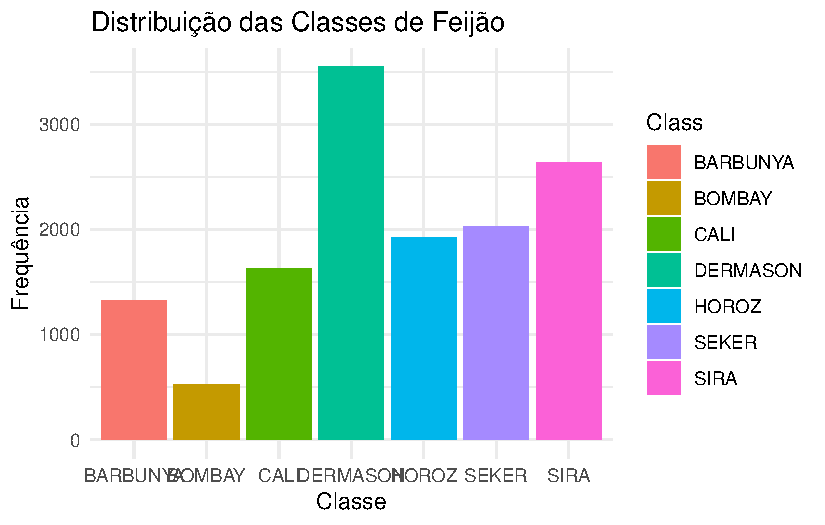
\includegraphics[keepaspectratio]{trabalho_files/figure-pdf/unnamed-chunk-3-1.pdf}}

\subsection{Glass Identification
Dataset}\label{glass-identification-dataset}

Esta base de dados foi criada para investigações de ciência forense,
onde fragmentos de vidro encontrados em cenas de crime podem ser usados
como evidência se corretamente identificados. A classificação se baseia
na composição química do vidro.

\begin{itemize}
\item
  Link para a fonte:
  \url{https://archive.ics.uci.edu/dataset/42/glass+identification}
\item
  Descrição Geral:
\item
  Número de Instâncias:~214.
\item
  Número de Atributos:~11 (10 atributos previsores e 1 atributo classe).
\item
  Atributo Classe:~\emph{Type\_of\_glass} (com 7 tipos possíveis, embora
  um deles não tenha instâncias na base, resultando em 6 classes
  efetivas).
\item
  Valores Ausentes:~A base de dados não possui valores ausentes.
\item
  Tipos de Atributos:~Os atributos são numéricos contínuos,
  representando o índice de refração (RI) e a porcentagem em peso de
  óxidos de diferentes elementos químicos (Sódio, Magnésio, Alumínio,
  etc.). Sendo eles:

  \begin{itemize}
  \item
    Id\_number: número identificador. à Discreto
  \item
    RI: Índice de refração. à Contínuo
  \item
    Na: Percentual em peso de sódio. à Contínuo
  \item
    Mg: Percentual em peso de magnésio. à Contínuo
  \item
    Al: Percentual em peso de alumínio. à Contínuo
  \item
    Si: Percentual em peso de silício. à Contínuo
  \item
    K: Percentual em peso de potássio. à Contínuo
  \item
    Ca: Percentual em peso de cálcio. à Contínuo
  \item
    Ba: Percentual em peso de bário. à Contínuo
  \item
    Fe: Percentual em peso de ferro. à Contínuo
  \item
    Classe:
  \end{itemize}
\end{itemize}

\begin{enumerate}
\def\labelenumi{\arabic{enumi}.}
\item
  Janelas de edifícios - \emph{float}
\item
  Janelas de edifícios - não \emph{float}
\item
  Janelas de veículos - \emph{float}
\item
  Janelas de veículos - não \emph{float} (sem amostras na base)
\item
  Recipientes
\item
  Utensílios de mesa
\item
  Faróis de veículos
\end{enumerate}

\textbf{Nota:} O termo ``\emph{float}'' se refere à técnica de produção
do vidro, onde uma camada fundida é nivelada sobre um banho de metal
líquido que resulta num vidro uniforme e de superfície regular. Seu
diferencial em relação ao método de ``não \emph{float}'' está no índice
de refração do material.

A base escolhida é desbalanceada, não contendo representação da classe 4
(janelas de veículos não \emph{float}), e contendo discrepâncias de
representação das demais classes, como ilustra o gráfico.

\begin{Shaded}
\begin{Highlighting}[]
\NormalTok{glass\_df }\OtherTok{\textless{}{-}} \FunctionTok{fread}\NormalTok{(}\StringTok{"glass.data"}\NormalTok{, }\AttributeTok{sep =} \StringTok{","}\NormalTok{, }\AttributeTok{header =} \ConstantTok{FALSE}\NormalTok{)}
\FunctionTok{colnames}\NormalTok{(glass\_df) }\OtherTok{\textless{}{-}} \FunctionTok{c}\NormalTok{(}
  \StringTok{"Id\_number"}\NormalTok{,}
  \StringTok{"RI"}\NormalTok{,  }\CommentTok{\# V2}
  \StringTok{"Na"}\NormalTok{,               }\CommentTok{\# V3}
  \StringTok{"Mg"}\NormalTok{,               }\CommentTok{\# V4}
  \StringTok{"Al"}\NormalTok{,               }\CommentTok{\# V5}
  \StringTok{"Si"}\NormalTok{,               }\CommentTok{\# V6}
  \StringTok{"K"}\NormalTok{,                }\CommentTok{\# V7}
  \StringTok{"Ca"}\NormalTok{,               }\CommentTok{\# V8}
  \StringTok{"Ba"}\NormalTok{,               }\CommentTok{\# V9}
  \StringTok{"Fe"}\NormalTok{,               }\CommentTok{\# V10}
  \StringTok{"Class"}             \CommentTok{\# V11}
\NormalTok{)}

\NormalTok{df }\OtherTok{\textless{}{-}}\NormalTok{ glass\_df }\SpecialCharTok{\%\textgreater{}\%} 
  \FunctionTok{group\_by}\NormalTok{(Class)}\SpecialCharTok{\%\textgreater{}\%} 
  \FunctionTok{count}\NormalTok{(}\FunctionTok{n}\NormalTok{()) }\SpecialCharTok{\%\textgreater{}\%} 
  \FunctionTok{mutate}\NormalTok{(}\AttributeTok{Class =} \FunctionTok{recode}\NormalTok{(Class,}
                        \StringTok{\textasciigrave{}}\AttributeTok{1}\StringTok{\textasciigrave{}} \OtherTok{=} \StringTok{"Janelas de edifícios (float)"}\NormalTok{,}
                        \StringTok{\textasciigrave{}}\AttributeTok{2}\StringTok{\textasciigrave{}} \OtherTok{=} \StringTok{"Janelas de edifícios (não{-}float)"}\NormalTok{,}
                        \StringTok{\textasciigrave{}}\AttributeTok{3}\StringTok{\textasciigrave{}} \OtherTok{=} \StringTok{"Janelas de veículos (float)"}\NormalTok{,}
                        \StringTok{\textasciigrave{}}\AttributeTok{4}\StringTok{\textasciigrave{}} \OtherTok{=} \StringTok{"Janelas de veículos (não{-}float)"}\NormalTok{,   }\CommentTok{\# não há amostras}
                        \StringTok{\textasciigrave{}}\AttributeTok{5}\StringTok{\textasciigrave{}} \OtherTok{=} \StringTok{"Recipientes"}\NormalTok{,}
                        \StringTok{\textasciigrave{}}\AttributeTok{6}\StringTok{\textasciigrave{}} \OtherTok{=} \StringTok{"Utensílios de mesa"}\NormalTok{,}
                        \StringTok{\textasciigrave{}}\AttributeTok{7}\StringTok{\textasciigrave{}} \OtherTok{=} \StringTok{"Faróis"}
\NormalTok{  )) }



\FunctionTok{ggplot}\NormalTok{(df, }\FunctionTok{aes}\NormalTok{(}\AttributeTok{x =}\NormalTok{ Class, }\AttributeTok{y =}\NormalTok{ n, }\AttributeTok{fill =}\NormalTok{ Class)) }\SpecialCharTok{+}
  \FunctionTok{geom\_col}\NormalTok{() }\SpecialCharTok{+}
  \FunctionTok{labs}\NormalTok{(}\AttributeTok{title =} \StringTok{"Distribuição das Classes de Vidro"}\NormalTok{,}
       \AttributeTok{x =} \StringTok{"Classe"}\NormalTok{,}
       \AttributeTok{y =} \StringTok{"Frequência"}\NormalTok{) }\SpecialCharTok{+}
  \FunctionTok{theme\_minimal}\NormalTok{()}
\end{Highlighting}
\end{Shaded}

\pandocbounded{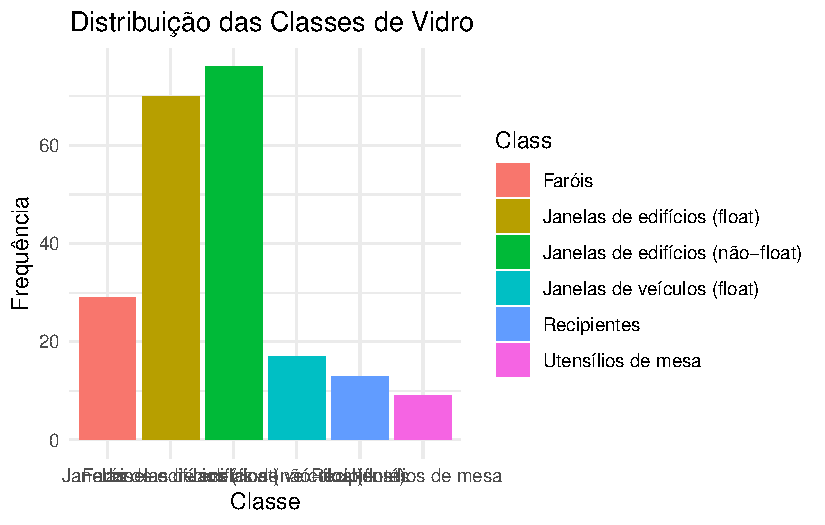
\includegraphics[keepaspectratio]{trabalho_files/figure-pdf/unnamed-chunk-4-1.pdf}}

\section{Ferramenta}\label{ferramenta}

Os experimentos foram realizados na linguagem \textbf{R}, em ambiente
RStudio, utilizando pacotes amplamente empregados na área de ciência de
dados. O pré-processamento e a manipulação das bases foram feitos
principalmente com o pacote \textbf{dplyr}, enquanto a execução dos
algoritmos contou com pacotes específicos: \textbf{class} (para o KNN),
\textbf{nnet} (para a Regressão Logística Multinomial), \textbf{rpart}
(para a Árvore de Decisão) e \textbf{caret} (para avaliação por meio da
matriz de confusão e cálculo da acurácia). Essa combinação de
ferramentas possibilitou a implementação consistente dos experimentos,
assegurando reprodutibilidade e clareza na comparação dos diferentes
algoritmos de classificação.

\section{Dry Bean Dataset}\label{dry-bean-dataset-1}

\subsection{Pré-processamento}\label{pruxe9-processamento}

Na base Dry Beans, que contém 13.611 instâncias e 16 atributos numéricos
derivados de medidas geométricas das sementes, foram aplicadas três
etapas principais de pré-processamento: amostragem, redução de
dimensionalidade e transformação de variáveis.

\subsubsection{Amostragem}\label{amostragem}

A amostragem foi considerada na base Dry Beans devido ao grande número
de instâncias (13.611), permitindo reduzir o custo computacional durante
os experimentos e possibilitando a execução de testes preliminares com
subconjuntos menores de dados, garantindo maior eficiência na comparação
entre classificadores. Optou-se pela amostragem estratificada, de modo a
preservar as proporções originais das sete classes de feijões no
subconjunto selecionado, o que se mostra essencial diante do
desbalanceamento existente entre as classes, já que algumas variedades
possuem muito mais instâncias que outras. Assim, essa estratégia
assegura que o conjunto reduzido de dados mantenha a diversidade e
representatividade necessárias para uma avaliação consistente do
desempenho dos algoritmos de classificação.

\begin{Shaded}
\begin{Highlighting}[]
\FunctionTok{set.seed}\NormalTok{(}\DecValTok{42}\NormalTok{) }\CommentTok{\# Reprodutibilidade}

\NormalTok{frac\_global }\OtherTok{\textless{}{-}} \FloatTok{0.03}  \CommentTok{\# define o tamanho da partição para 3\% do dataset}

\NormalTok{bean\_df\_bal }\OtherTok{\textless{}{-}}\NormalTok{ bean\_df }\SpecialCharTok{\%\textgreater{}\%}
  \FunctionTok{group\_by}\NormalTok{(Class) }\SpecialCharTok{\%\textgreater{}\%} 
  \FunctionTok{slice\_sample}\NormalTok{(}\AttributeTok{prop =}\NormalTok{ frac\_global) }\SpecialCharTok{\%\textgreater{}\%} \CommentTok{\# realiza a partiçao da amostragem}
  \FunctionTok{ungroup}\NormalTok{()}


\CommentTok{\# Garantia de manutenção das proporções}
\NormalTok{df }\OtherTok{\textless{}{-}}\NormalTok{ bean\_df\_bal }\SpecialCharTok{\%\textgreater{}\%} 
  \FunctionTok{group\_by}\NormalTok{(Class)}\SpecialCharTok{\%\textgreater{}\%} 
  \FunctionTok{count}\NormalTok{(}\FunctionTok{n}\NormalTok{())}

\FunctionTok{ggplot}\NormalTok{(df, }\FunctionTok{aes}\NormalTok{(}\AttributeTok{x =}\NormalTok{ Class, }\AttributeTok{y =}\NormalTok{ n, }\AttributeTok{fill =}\NormalTok{ Class)) }\SpecialCharTok{+}
  \FunctionTok{geom\_col}\NormalTok{() }\SpecialCharTok{+}
  \FunctionTok{labs}\NormalTok{(}\AttributeTok{title =} \StringTok{"Distribuição das Classes de Feijão"}\NormalTok{,}
       \AttributeTok{x =} \StringTok{"Classe"}\NormalTok{,}
       \AttributeTok{y =} \StringTok{"Frequência"}\NormalTok{) }\SpecialCharTok{+}
  \FunctionTok{theme\_minimal}\NormalTok{()}
\end{Highlighting}
\end{Shaded}

\pandocbounded{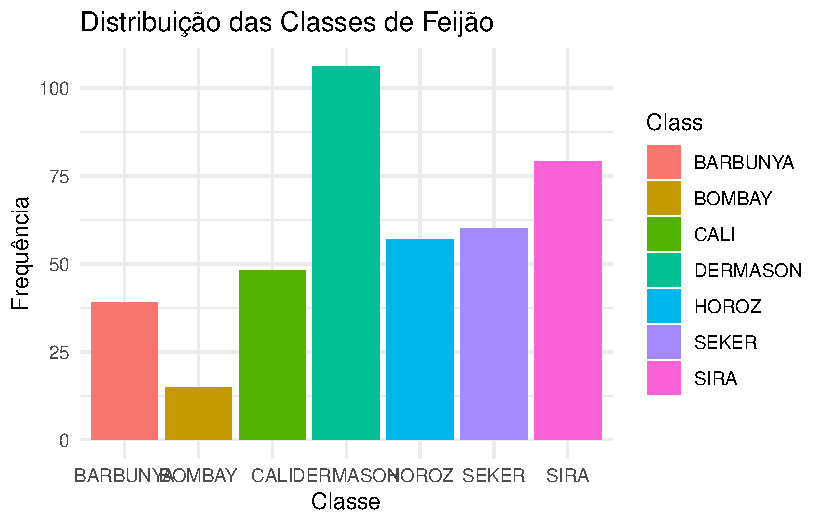
\includegraphics[keepaspectratio]{trabalho_files/figure-pdf/unnamed-chunk-5-1.pdf}}

\subsubsection{Estratégia de Divisão da Base de
Dados}\label{estratuxe9gia-de-divisuxe3o-da-base-de-dados}

Adotou-se a estratégia de divisão Holdout para a separação dos dados em
treino e teste. Essa técnica consiste em particionar a base em dois
subconjuntos mutuamente exclusivos: um destinado ao treinamento do
modelo e outro reservado para a sua avaliação. Optou-se por utilizar
aproximadamente 2/3 dos dados para o treino e 1/3 para o teste, de modo
a garantir que o classificador tivesse acesso a uma quantidade
suficiente de instâncias para o aprendizado, ao mesmo tempo em que fosse
avaliado em exemplos não vistos durante o treinamento. Essa abordagem
permite estimar o desempenho do modelo de forma direta e eficiente,
sendo amplamente utilizada em cenários com bases de dados de tamanho
moderado.

\begin{Shaded}
\begin{Highlighting}[]
\FunctionTok{set.seed}\NormalTok{(}\DecValTok{42}\NormalTok{) }\CommentTok{\# Reprodutibilidade}

\NormalTok{idx\_treino\_bean }\OtherTok{\textless{}{-}}\NormalTok{ bean\_df\_bal }\SpecialCharTok{\%\textgreater{}\%}
  \FunctionTok{mutate}\NormalTok{(}\AttributeTok{row\_id =}\NormalTok{ dplyr}\SpecialCharTok{::}\FunctionTok{row\_number}\NormalTok{()) }\SpecialCharTok{\%\textgreater{}\%}
  \FunctionTok{group\_by}\NormalTok{(Class) }\SpecialCharTok{\%\textgreater{}\%}
  \FunctionTok{slice\_sample}\NormalTok{(}\AttributeTok{prop =} \DecValTok{2}\SpecialCharTok{/}\DecValTok{3}\NormalTok{) }\SpecialCharTok{\%\textgreater{}\%} \CommentTok{\# Realiza a partição da base para treino e teste}
  \FunctionTok{pull}\NormalTok{(row\_id)}
\end{Highlighting}
\end{Shaded}

\subsubsection{Redução de
Dimensionalidade}\label{reduuxe7uxe3o-de-dimensionalidade}

Na redução de dimensionalidade, observou-se que diversos atributos da
base são derivados de outros já existentes, apresentando, portanto,
redundância. Por exemplo, o atributo \emph{AspectRation} é calculado a
partir da razão entre \emph{MajorAxisLength} e \emph{MinorAxisLength},
enquanto \emph{Roundness} e \emph{Compactness} utilizam \emph{Area} e
\emph{Perimeter} em suas fórmulas. Dessa forma, optou-se por manter os
atributos derivados e remover os fundamentais. Essa abordagem preserva a
informação essencial em métricas normalizadas e reduz a redundância
entre variáveis, conforme ilustrado na tabela apresentada nesta seção.

\begin{Shaded}
\begin{Highlighting}[]
\CommentTok{\# Retirada das colunas fundamentais }
\NormalTok{bean\_df\_bal }\OtherTok{\textless{}{-}}\NormalTok{ bean\_df\_bal }\SpecialCharTok{\%\textgreater{}\%} 
  \FunctionTok{select}\NormalTok{(}\SpecialCharTok{{-}}\FunctionTok{c}\NormalTok{(}\StringTok{"MinorAxisLength"}\NormalTok{, }\StringTok{"MajorAxisLength"}\NormalTok{, }\StringTok{"Area"}\NormalTok{, }\StringTok{"Perimeter"}\NormalTok{, }\StringTok{"ConvexArea"}\NormalTok{))}
\end{Highlighting}
\end{Shaded}

\subsubsection{Normalização}\label{normalizauxe7uxe3o}

No processo de pré-processamento dos dados, adotou-se a normalização das
variáveis preditoras, etapa fundamental para a execução de algoritmos de
classificação baseados em medidas de distância e em modelos estatísticos
multivariados. Foram utilizadas duas abordagens distintas conforme a
necessidade de cada algoritmo: a normalização por re-escala e a
padronização. A normalização por re-escala transforma os atributos para
um intervalo comum, tipicamente {[}0, 1{]}, evitando que variáveis com
grande amplitude numérica dominem o cálculo das distâncias, como ocorre
no KNN. Já a padronização converte cada atributo para média zero e
desvio-padrão unitário, garantindo comparabilidade em algoritmos como a
regressão logística, que assumem variáveis centradas e na mesma escala.
Dessa forma, a aplicação dessas técnicas assegurou que todos os
atributos contribuíssem de forma equilibrada no processo de
classificação, aumentando a robustez e a interpretabilidade dos
resultados obtidos.

\paragraph{Re-escalar}\label{re-escalar}

Normalização utilizada para o algoritmo KNN.

\begin{Shaded}
\begin{Highlighting}[]
\NormalTok{min\_max\_normalization }\OtherTok{\textless{}{-}} \ControlFlowTok{function}\NormalTok{(x) \{}
  \FunctionTok{return}\NormalTok{ ((x }\SpecialCharTok{{-}} \FunctionTok{min}\NormalTok{(x)) }\SpecialCharTok{/}\NormalTok{ (}\FunctionTok{max}\NormalTok{(x) }\SpecialCharTok{{-}} \FunctionTok{min}\NormalTok{(x)))}
\NormalTok{\}}

\CommentTok{\# Aplicando normalização (re{-}escala) nas colunas numéricas}
\NormalTok{bean\_df\_res }\OtherTok{\textless{}{-}}\NormalTok{ bean\_df\_bal }\SpecialCharTok{\%\textgreater{}\%} 
  \FunctionTok{mutate}\NormalTok{(}\FunctionTok{across}\NormalTok{(}\FunctionTok{c}\NormalTok{(}\StringTok{"AspectRation"}\NormalTok{, }\StringTok{"Eccentricity"}\NormalTok{, }\StringTok{"EquivDiameter"}\NormalTok{, }\StringTok{"Extent"}\NormalTok{, }\StringTok{"Solidity"}\NormalTok{, }\StringTok{"roundness"}\NormalTok{, }\StringTok{"Compactness"}\NormalTok{, }\StringTok{"ShapeFactor1"}\NormalTok{, }\StringTok{"ShapeFactor2"}\NormalTok{, }\StringTok{"ShapeFactor3"}\NormalTok{, }\StringTok{"ShapeFactor4"}\NormalTok{), min\_max\_normalization))}

\NormalTok{bean\_df\_res }\SpecialCharTok{\%\textgreater{}\%} 
  \FunctionTok{select}\NormalTok{(}
\NormalTok{    AspectRation, }
\NormalTok{    Eccentricity, }
\NormalTok{    EquivDiameter, }
\NormalTok{    Extent, }
\NormalTok{    Solidity, }
\NormalTok{    roundness, }
\NormalTok{    Compactness, }
\NormalTok{    ShapeFactor1, }
\NormalTok{    ShapeFactor2, }
\NormalTok{    ShapeFactor3, }
\NormalTok{    ShapeFactor4}
\NormalTok{  )}
\end{Highlighting}
\end{Shaded}

\begin{verbatim}
# A tibble: 404 x 11
   AspectRation Eccentricity EquivDiameter Extent Solidity roundness
          <dbl>        <dbl>         <dbl>  <dbl>    <dbl>     <dbl>
 1        0.280        0.640         0.371  0.548    0.832     0.644
 2        0.399        0.753         0.339  0.526    0.685     0.360
 3        0.301        0.663         0.454  0.445    0.766     0.396
 4        0.391        0.746         0.437  0.763    0.608     0.191
 5        0.174        0.493         0.479  0.668    0.840     0.716
 6        0.410        0.762         0.452  0.537    0.633     0.337
 7        0.376        0.735         0.377  0.537    0.791     0.524
 8        0.368        0.727         0.262  0.543    0.766     0.556
 9        0.346        0.708         0.446  0.788    0.790     0.592
10        0.286        0.648         0.243  0.864    0.932     0.868
# i 394 more rows
# i 5 more variables: Compactness <dbl>, ShapeFactor1 <dbl>,
#   ShapeFactor2 <dbl>, ShapeFactor3 <dbl>, ShapeFactor4 <dbl>
\end{verbatim}

\paragraph{Padronização}\label{padronizauxe7uxe3o}

Normalização utilizada para o algoritmo Regressão Logística.

\begin{Shaded}
\begin{Highlighting}[]
\NormalTok{padronization\_norm }\OtherTok{\textless{}{-}} \ControlFlowTok{function}\NormalTok{(x)\{}
  \FunctionTok{return}\NormalTok{((x}\SpecialCharTok{{-}}\FunctionTok{mean}\NormalTok{(x))}\SpecialCharTok{/}\FunctionTok{sd}\NormalTok{(x))}
\NormalTok{\}}

\CommentTok{\# Aplicando normalização (padronização) nas colunas numéricas}
\NormalTok{bean\_df\_pad }\OtherTok{\textless{}{-}}\NormalTok{ bean\_df\_res }\SpecialCharTok{\%\textgreater{}\%} 
  \FunctionTok{mutate}\NormalTok{(}\FunctionTok{across}\NormalTok{(}\FunctionTok{c}\NormalTok{(}\StringTok{"AspectRation"}\NormalTok{, }\StringTok{"Eccentricity"}\NormalTok{, }\StringTok{"EquivDiameter"}\NormalTok{, }\StringTok{"Extent"}\NormalTok{, }\StringTok{"Solidity"}\NormalTok{, }\StringTok{"roundness"}\NormalTok{, }\StringTok{"Compactness"}\NormalTok{, }\StringTok{"ShapeFactor1"}\NormalTok{, }\StringTok{"ShapeFactor2"}\NormalTok{, }\StringTok{"ShapeFactor3"}\NormalTok{, }\StringTok{"ShapeFactor4"}\NormalTok{), padronization\_norm))}

\NormalTok{bean\_df\_pad }\SpecialCharTok{\%\textgreater{}\%} 
  \FunctionTok{select}\NormalTok{(}
\NormalTok{    AspectRation, }
\NormalTok{    Eccentricity, }
\NormalTok{    EquivDiameter, }
\NormalTok{    Extent, }
\NormalTok{    Solidity, }
\NormalTok{    roundness, }
\NormalTok{    Compactness, }
\NormalTok{    ShapeFactor1, }
\NormalTok{    ShapeFactor2, }
\NormalTok{    ShapeFactor3, }
\NormalTok{    ShapeFactor4}
\NormalTok{  )}
\end{Highlighting}
\end{Shaded}

\begin{verbatim}
# A tibble: 404 x 11
   AspectRation Eccentricity EquivDiameter  Extent Solidity roundness
          <dbl>        <dbl>         <dbl>   <dbl>    <dbl>     <dbl>
 1      -0.649       -0.425         0.712  -0.730    -0.214   -0.415 
 2      -0.0268       0.233         0.514  -0.851    -1.72    -2.11  
 3      -0.540       -0.291         1.22   -1.30     -0.892   -1.89  
 4      -0.0723       0.193         1.12    0.448    -2.52    -3.11  
 5      -1.20        -1.28          1.38   -0.0765   -0.132    0.0115
 6       0.0297       0.282         1.21   -0.793    -2.26    -2.25  
 7      -0.147        0.125         0.751  -0.790    -0.636   -1.13  
 8      -0.193        0.0812        0.0384 -0.760    -0.888   -0.941 
 9      -0.305       -0.0301        1.18    0.584    -0.642   -0.723 
10      -0.616       -0.383        -0.0779  1.00      0.815    0.919 
# i 394 more rows
# i 5 more variables: Compactness <dbl>, ShapeFactor1 <dbl>,
#   ShapeFactor2 <dbl>, ShapeFactor3 <dbl>, ShapeFactor4 <dbl>
\end{verbatim}

\subsection{Algoritmos}\label{algoritmos}

\subsubsection{Árvore de Decisão}\label{uxe1rvore-de-decisuxe3o}

\begin{Shaded}
\begin{Highlighting}[]
\FunctionTok{set.seed}\NormalTok{(}\DecValTok{42}\NormalTok{)  }\CommentTok{\# Reprodutibilidade}

\NormalTok{bean\_df\_bal}\SpecialCharTok{$}\NormalTok{Class }\OtherTok{\textless{}{-}} \FunctionTok{as.factor}\NormalTok{(bean\_df\_bal}\SpecialCharTok{$}\NormalTok{Class) }\CommentTok{\# Garante que a classe é factor}

\CommentTok{\# Armazena a parte de treino e base separada em idx\_treino\_bean}
\NormalTok{train\_dt\_bean }\OtherTok{\textless{}{-}}\NormalTok{ bean\_df\_bal[idx\_treino\_bean, ]}
\NormalTok{test\_dt\_bean  }\OtherTok{\textless{}{-}}\NormalTok{ bean\_df\_bal[}\SpecialCharTok{{-}}\NormalTok{idx\_treino\_bean, ]}

\CommentTok{\# Fórmula: alvo \textasciitilde{} todos os preditores}
\NormalTok{form\_dt\_bean }\OtherTok{\textless{}{-}} \FunctionTok{reformulate}\NormalTok{(}\FunctionTok{setdiff}\NormalTok{(}\FunctionTok{names}\NormalTok{(train\_dt\_bean), }\StringTok{\textquotesingle{}Class\textquotesingle{}}\NormalTok{), }\AttributeTok{response =} \StringTok{\textquotesingle{}Class\textquotesingle{}}\NormalTok{)}

\CommentTok{\# Executar Árvore de Decisão para cp (p1) = 0.05}
\NormalTok{cp\_p1\_dt\_bean  }\OtherTok{\textless{}{-}} \FunctionTok{rpart}\NormalTok{(form\_dt\_bean, }\AttributeTok{data =}\NormalTok{ train\_dt\_bean, }\AttributeTok{method =} \StringTok{"class"}\NormalTok{, }\AttributeTok{control =} \FunctionTok{rpart.control}\NormalTok{(}\AttributeTok{cp =} \FloatTok{0.05}\NormalTok{))}
\NormalTok{pred\_p1\_dt\_bean  }\OtherTok{\textless{}{-}} \FunctionTok{predict}\NormalTok{(cp\_p1\_dt\_bean,  }\AttributeTok{newdata =}\NormalTok{ test\_dt\_bean, }\AttributeTok{type =} \StringTok{"class"}\NormalTok{)}

\CommentTok{\# Executar Árvore de Decisão para cp (p2) = 0.001}
\NormalTok{cp\_p2\_dt\_bean }\OtherTok{\textless{}{-}} \FunctionTok{rpart}\NormalTok{(form\_dt\_bean, }\AttributeTok{data =}\NormalTok{ train\_dt\_bean, }\AttributeTok{method =} \StringTok{"class"}\NormalTok{, }\AttributeTok{control =} \FunctionTok{rpart.control}\NormalTok{(}\AttributeTok{cp =} \FloatTok{0.001}\NormalTok{))}
\NormalTok{pred\_p2\_dt\_bean }\OtherTok{\textless{}{-}} \FunctionTok{predict}\NormalTok{(cp\_p2\_dt\_bean, }\AttributeTok{newdata =}\NormalTok{ test\_dt\_bean, }\AttributeTok{type =} \StringTok{"class"}\NormalTok{)}
\end{Highlighting}
\end{Shaded}

\subsubsection{KNN}\label{knn}

\begin{Shaded}
\begin{Highlighting}[]
\FunctionTok{set.seed}\NormalTok{(}\DecValTok{42}\NormalTok{) }\CommentTok{\# Reprodutibilidade}

\NormalTok{bean\_df\_res}\SpecialCharTok{$}\NormalTok{Class }\OtherTok{\textless{}{-}} \FunctionTok{as.factor}\NormalTok{(bean\_df\_res}\SpecialCharTok{$}\NormalTok{Class) }\CommentTok{\# Garante que a classe é factor}

\CommentTok{\# Armazena a parte de treino e base separada em idx\_treino\_bean}
\NormalTok{train\_knn\_bean }\OtherTok{\textless{}{-}}\NormalTok{ bean\_df\_res[idx\_treino\_bean, ]}
\NormalTok{test\_knn\_bean  }\OtherTok{\textless{}{-}}\NormalTok{ bean\_df\_res[}\SpecialCharTok{{-}}\NormalTok{idx\_treino\_bean, ]}

\CommentTok{\# Matriz de preditores (x) e vetores de classe (y)}
\NormalTok{X\_train\_knn\_bean }\OtherTok{\textless{}{-}}\NormalTok{ train\_knn\_bean }\SpecialCharTok{\%\textgreater{}\%}
  \FunctionTok{select}\NormalTok{(}\SpecialCharTok{{-}}\FunctionTok{all\_of}\NormalTok{(}\StringTok{\textquotesingle{}Class\textquotesingle{}}\NormalTok{)) }\SpecialCharTok{\%\textgreater{}\%} 
  \FunctionTok{as.data.frame}\NormalTok{()}

\NormalTok{X\_test\_knn\_bean  }\OtherTok{\textless{}{-}}\NormalTok{ test\_knn\_bean }\SpecialCharTok{\%\textgreater{}\%} 
  \FunctionTok{select}\NormalTok{(}\SpecialCharTok{{-}}\FunctionTok{all\_of}\NormalTok{(}\StringTok{\textquotesingle{}Class\textquotesingle{}}\NormalTok{)) }\SpecialCharTok{\%\textgreater{}\%} 
  \FunctionTok{as.data.frame}\NormalTok{()}

\NormalTok{y\_train\_knn\_bean }\OtherTok{\textless{}{-}}\NormalTok{ train\_knn\_bean}\SpecialCharTok{$}\NormalTok{Class}
\NormalTok{y\_test\_knn\_bean }\OtherTok{\textless{}{-}}\NormalTok{ test\_knn\_bean}\SpecialCharTok{$}\NormalTok{Class}

\FunctionTok{stopifnot}\NormalTok{(}\FunctionTok{is.factor}\NormalTok{(y\_train\_knn\_bean), }\FunctionTok{is.factor}\NormalTok{(y\_test\_knn\_bean)) }\CommentTok{\# Verifica se todos os valores são factor (exigido pelo KNN)}
\FunctionTok{stopifnot}\NormalTok{(}\FunctionTok{all}\NormalTok{(}\FunctionTok{sapply}\NormalTok{(X\_train\_knn\_bean, is.numeric)), }\FunctionTok{all}\NormalTok{(}\FunctionTok{sapply}\NormalTok{(X\_test\_knn\_bean, is.numeric))) }\CommentTok{\# Verifica se todos os valores são numéricos (exigido pelo KNN)}

\CommentTok{\# Executar KNN para k (p1) = 3}
\NormalTok{k\_p1\_knn\_bean }\OtherTok{\textless{}{-}} \DecValTok{3} \CommentTok{\# Define a quantidade de K{-}vizinhos mais próximos}

\NormalTok{pred\_k\_p1\_knn\_bean }\OtherTok{\textless{}{-}} \FunctionTok{knn}\NormalTok{(}
  \AttributeTok{train =}\NormalTok{ X\_train\_knn\_bean,   }\CommentTok{\# base de treino (preditores)}
  \AttributeTok{test  =}\NormalTok{ X\_test\_knn\_bean,    }\CommentTok{\# base de teste  (preditores)}
  \AttributeTok{cl    =}\NormalTok{ y\_train\_knn\_bean,   }\CommentTok{\# classes de treino (factor)}
  \AttributeTok{k     =}\NormalTok{ k\_p1\_knn\_bean       }\CommentTok{\# número de vizinhos}
\NormalTok{)}

\CommentTok{\# Executar KNN para k (p2) = 5}
\NormalTok{k\_p2\_knn\_bean }\OtherTok{\textless{}{-}} \DecValTok{5} \CommentTok{\# Define a quantidade de K{-}vizinhos mais próximos}

\NormalTok{pred\_k\_p2\_knn\_bean }\OtherTok{\textless{}{-}} \FunctionTok{knn}\NormalTok{(}
  \AttributeTok{train =}\NormalTok{ X\_train\_knn\_bean,   }\CommentTok{\# base de treino (preditores)}
  \AttributeTok{test  =}\NormalTok{ X\_test\_knn\_bean,    }\CommentTok{\# base de teste  (preditores)}
  \AttributeTok{cl    =}\NormalTok{ y\_train\_knn\_bean,   }\CommentTok{\# classes de treino (factor)}
  \AttributeTok{k     =}\NormalTok{ k\_p2\_knn\_bean        }\CommentTok{\# número de vizinhos}
\NormalTok{)}
\end{Highlighting}
\end{Shaded}

\subsubsection{Regressão Logística}\label{regressuxe3o-loguxedstica}

\paragraph{Metodologia do Modelo de Regressão Logística
Multinomial}\label{metodologia-do-modelo-de-regressuxe3o-loguxedstica-multinomial}

A regressão logística multinomial é um modelo estatístico utilizado para
prever variáveis dependentes categóricas com mais de duas classes. No
presente estudo, este modelo foi aplicado para classificar amostras de
acordo com suas características, conforme descrito a seguir.

\begin{enumerate}
\def\labelenumi{\arabic{enumi}.}
\item
  \textbf{Preparação dos dados}

  Inicialmente, os dados foram organizados de forma a conter as
  variáveis independentes (atributos) e a variável resposta (classe).
  Uma das classes foi definida automaticamente como referência, servindo
  de base para a comparação com as demais.
\item
  \textbf{Definição inicial dos parâmetros}

  O modelo associa pesos (parâmetros) a cada variável em cada classe.
  Esses pesos indicam a intensidade e a direção da influência de uma
  característica sobre a probabilidade de pertencimento a determinada
  classe. No início do processo, os valores dos pesos são atribuídos de
  forma arbitrária, próximos de zero.
\item
  \textbf{Cálculo das probabilidades}

  A cada iteração, os dados são processados e o modelo gera pontuações
  para cada classe. Essas pontuações são transformadas em probabilidades
  através de uma função de normalização, garantindo que a soma das
  probabilidades de todas as classes seja igual a 100\%.
\item
  \textbf{Comparação com os valores reais}

  As probabilidades estimadas são comparadas com os valores observados
  na base de dados. O modelo verifica o grau de acerto e erro das
  previsões em relação às classes reais atribuídas a cada observação.
\item
  \textbf{Ajuste dos pesos}

  Com base na diferença entre valores previstos e reais, os pesos
  associados às variáveis são ajustados. Esse processo corrige a
  influência das variáveis, reforçando aquelas que ajudam na
  classificação correta e reduzindo o impacto daquelas que conduzem a
  erros.
\item
  \textbf{Iteração e convergência}

  O ciclo de cálculo de probabilidades, comparação com os valores reais
  e ajuste dos pesos é repetido sucessivamente. O processo segue até que
  os ajustes se tornem mínimos, caracterizando a convergência do modelo.
  Nesse ponto, considera-se que o modelo aprendeu a relação entre
  atributos e classes.
\item
  \textbf{Modelo final e aplicação}

  Após a convergência, o modelo retém um conjunto de pesos ajustados
  para cada classe. Esses parâmetros permitem identificar quais
  variáveis exercem maior influência na diferenciação entre as classes.
  Em novos dados, o modelo aplica os pesos, calcula as probabilidades de
  cada classe e retorna como previsão a classe com maior probabilidade
  associada.
\end{enumerate}

O funcionamento da regressão logística multinomial pode ser resumido
como um processo de aprendizado iterativo: o modelo começa com
estimativas iniciais, compara suas previsões com os resultados
observados, ajusta seus parâmetros e repete o processo até estabilizar.
Dessa forma, consegue capturar padrões nos dados e utilizá-los para
realizar classificações em situações~futuras.

\begin{Shaded}
\begin{Highlighting}[]
\FunctionTok{set.seed}\NormalTok{(}\DecValTok{42}\NormalTok{)}

\CommentTok{\# Armazena a parte de treino e base separada em idx\_treino\_bean}
\NormalTok{train\_rl\_bean }\OtherTok{\textless{}{-}}\NormalTok{ bean\_df\_pad[idx\_treino\_bean, ]}
\NormalTok{test\_rl\_bean  }\OtherTok{\textless{}{-}}\NormalTok{ bean\_df\_pad[}\SpecialCharTok{{-}}\NormalTok{idx\_treino\_bean, ]}


\NormalTok{model\_rl\_bean }\OtherTok{\textless{}{-}} \FunctionTok{multinom}\NormalTok{(Class }\SpecialCharTok{\textasciitilde{}}\NormalTok{ AspectRation }\SpecialCharTok{+}\NormalTok{ Eccentricity }\SpecialCharTok{+}\NormalTok{ EquivDiameter }\SpecialCharTok{+}\NormalTok{ Extent }\SpecialCharTok{+}\NormalTok{ Solidity }\SpecialCharTok{+}\NormalTok{ roundness }\SpecialCharTok{+}\NormalTok{ Compactness }\SpecialCharTok{+}\NormalTok{ ShapeFactor1 }\SpecialCharTok{+}\NormalTok{ ShapeFactor2 }\SpecialCharTok{+}\NormalTok{ ShapeFactor3 }\SpecialCharTok{+}\NormalTok{ ShapeFactor4, }\AttributeTok{data =}\NormalTok{ train\_rl\_bean)}
\end{Highlighting}
\end{Shaded}

\begin{verbatim}
# weights:  91 (72 variable)
initial  value 521.503920 
iter  10 value 132.886753
iter  20 value 57.469306
iter  30 value 28.454307
iter  40 value 20.878223
iter  50 value 19.399664
iter  60 value 18.450299
iter  70 value 17.078242
iter  80 value 16.334450
iter  90 value 16.066841
iter 100 value 15.976636
final  value 15.976636 
stopped after 100 iterations
\end{verbatim}

\begin{Shaded}
\begin{Highlighting}[]
\NormalTok{coefs }\OtherTok{\textless{}{-}} \FunctionTok{summary}\NormalTok{(model\_rl\_bean)}\SpecialCharTok{$}\NormalTok{coefficients }\CommentTok{\# pesos atribuidos a cada atributo de acordo com a classe}
 
\NormalTok{prediction\_rl\_bean }\OtherTok{\textless{}{-}} \FunctionTok{predict}\NormalTok{(model\_rl\_bean, }\AttributeTok{newdata =}\NormalTok{ test\_rl\_bean)}
\end{Highlighting}
\end{Shaded}

Para testagem do desempenho do modelo com outros parâmetros, testaremos
o treinamento apenas com os atributos mais relevantes para cada classe,
baseado nos pesos a elas atribuídos.

\begin{Shaded}
\begin{Highlighting}[]
\CommentTok{\# Converter os coeficientes em um data frame para facilitar a manipulação}
\NormalTok{coefs\_df }\OtherTok{\textless{}{-}} \FunctionTok{as.data.frame}\NormalTok{(coefs)}
\CommentTok{\# Calcular os coeficientes absolutos}
\NormalTok{coefs\_abs }\OtherTok{\textless{}{-}} \FunctionTok{abs}\NormalTok{(coefs\_df)}
\CommentTok{\# Para cada variável (linha), pegar o maior valor absoluto e associar à variável}
\NormalTok{max\_values }\OtherTok{\textless{}{-}} \FunctionTok{apply}\NormalTok{(coefs\_abs, }\DecValTok{1}\NormalTok{, max)}
\CommentTok{\# Agora associamos os valores máximos às variáveis (colunas)}
\NormalTok{max\_vars }\OtherTok{\textless{}{-}} \FunctionTok{apply}\NormalTok{(coefs\_abs, }\DecValTok{1}\NormalTok{, }\ControlFlowTok{function}\NormalTok{(x) }\FunctionTok{names}\NormalTok{(x)[}\FunctionTok{which.max}\NormalTok{(x)])}
\CommentTok{\# Criar um data frame para mostrar os atributos associados aos maiores valores}
\NormalTok{important\_vars }\OtherTok{\textless{}{-}} \FunctionTok{data.frame}\NormalTok{(}\AttributeTok{Variable =}\NormalTok{ max\_vars, }\AttributeTok{MaxValue =}\NormalTok{ max\_values)}
\CommentTok{\# Ordenar pelas variáveis com maior coeficiente absoluto}
\NormalTok{important\_vars\_sorted }\OtherTok{\textless{}{-}}\NormalTok{ important\_vars[}\FunctionTok{order}\NormalTok{(}\SpecialCharTok{{-}}\NormalTok{important\_vars}\SpecialCharTok{$}\NormalTok{MaxValue), ]}
\CommentTok{\# Mostrar as variáveis mais importantes}
\FunctionTok{head}\NormalTok{(important\_vars\_sorted)}
\end{Highlighting}
\end{Shaded}

\begin{verbatim}
              Variable  MaxValue
BOMBAY   EquivDiameter 134.16990
HOROZ     AspectRation 100.76669
DERMASON  ShapeFactor1  97.92946
CALI      ShapeFactor1  86.57764
SEKER     AspectRation  73.02434
SIRA     EquivDiameter  72.88013
\end{verbatim}

\begin{Shaded}
\begin{Highlighting}[]
\NormalTok{model\_rl\_bean\_less\_att }\OtherTok{\textless{}{-}} \FunctionTok{multinom}\NormalTok{(Class }\SpecialCharTok{\textasciitilde{}}\NormalTok{  EquivDiameter }\SpecialCharTok{+}\NormalTok{ roundness }\SpecialCharTok{+}\NormalTok{ ShapeFactor1 }\SpecialCharTok{+}\NormalTok{ ShapeFactor4, }\AttributeTok{data =}\NormalTok{ train\_rl\_bean)}
\end{Highlighting}
\end{Shaded}

\begin{verbatim}
# weights:  42 (30 variable)
initial  value 521.503920 
iter  10 value 130.809544
iter  20 value 58.402316
iter  30 value 40.529394
iter  40 value 39.089893
iter  50 value 38.178091
iter  60 value 37.939610
iter  70 value 37.868220
iter  80 value 37.781302
iter  90 value 37.742867
iter 100 value 37.710568
final  value 37.710568 
stopped after 100 iterations
\end{verbatim}

\begin{Shaded}
\begin{Highlighting}[]
\NormalTok{coefs\_bean\_less\_att }\OtherTok{\textless{}{-}} \FunctionTok{summary}\NormalTok{(model\_rl\_bean\_less\_att)}\SpecialCharTok{$}\NormalTok{coefficients }\CommentTok{\# pesos atribuidos a cada atributo de acordo com a classe}
\NormalTok{prediction\_rl\_bean\_less\_att }\OtherTok{\textless{}{-}} \FunctionTok{predict}\NormalTok{(model\_rl\_bean\_less\_att, }\AttributeTok{newdata =}\NormalTok{ test\_rl\_bean)}
\end{Highlighting}
\end{Shaded}

\subsection{Medidas de Avaliação}\label{medidas-de-avaliauxe7uxe3o}

Para a avaliação dos classificadores, foram utilizadas duas medidas
principais: a matriz de confusão e a acurácia. A matriz de confusão
consiste em uma tabela que organiza as previsões do modelo em relação
aos valores reais, discriminando corretamente os acertos e os erros de
classificação para cada classe. A acurácia, por sua vez, expressa a
proporção de instâncias corretamente classificadas pelo modelo em
relação ao total de instâncias avaliadas, sendo calculada pela fórmula:

Acurácia = (TP + TN) / (TP + TN + FP + FN)

em que TP (true positive) e TN (true negative) representam as previsões
corretas, enquanto FP (false positive) e FN (false negative)
correspondem às classificações incorretas.

\begin{Shaded}
\begin{Highlighting}[]
\CommentTok{\# {-}{-}{-}{-}{-}{-}{-}{-}{-}{-}{-}{-}{-}{-}{-}{-}{-}{-}{-}{-} Árvore de Decisão {-}{-}{-}{-}{-}{-}{-}{-}{-}{-}{-}{-}{-}{-}{-}{-}{-}{-}{-}{-}}

\CommentTok{\# Avaliar | cp (p1) = 0.05}
\NormalTok{conf\_p1\_dt\_bean }\OtherTok{\textless{}{-}} \FunctionTok{confusionMatrix}\NormalTok{(pred\_p1\_dt\_bean,test\_dt\_bean}\SpecialCharTok{$}\NormalTok{Class)}
\NormalTok{acc\_p1\_dt\_bean }\OtherTok{\textless{}{-}} \FunctionTok{mean}\NormalTok{(pred\_p1\_dt\_bean }\SpecialCharTok{==}\NormalTok{ test\_dt\_bean}\SpecialCharTok{$}\NormalTok{Class)}

\CommentTok{\# Avaliar | cp (p2) = 0.001}
\NormalTok{conf\_p2\_dt\_bean }\OtherTok{\textless{}{-}} \FunctionTok{confusionMatrix}\NormalTok{(pred\_p2\_dt\_bean,test\_dt\_bean}\SpecialCharTok{$}\NormalTok{Class)}
\NormalTok{acc\_p2\_dt\_bean }\OtherTok{\textless{}{-}} \FunctionTok{mean}\NormalTok{(pred\_p2\_dt\_bean }\SpecialCharTok{==}\NormalTok{ test\_dt\_bean}\SpecialCharTok{$}\NormalTok{Class)}

\FunctionTok{print}\NormalTok{(}\FunctionTok{paste}\NormalTok{(}\StringTok{"A acurácia do dataset DRY BEAN é superior com cp = "}\NormalTok{, }
            \FunctionTok{ifelse}\NormalTok{(acc\_p1\_dt\_bean }\SpecialCharTok{\textgreater{}}\NormalTok{ acc\_p2\_dt\_bean, }\FloatTok{0.05}\NormalTok{, }\FloatTok{0.001}\NormalTok{)}
\NormalTok{            )}
\NormalTok{      )}
\end{Highlighting}
\end{Shaded}

\begin{verbatim}
[1] "A acurácia do dataset DRY BEAN é superior com cp =  0.001"
\end{verbatim}

\begin{Shaded}
\begin{Highlighting}[]
\CommentTok{\# {-}{-}{-}{-}{-}{-}{-}{-}{-}{-}{-}{-}{-}{-}{-}{-}{-}{-}{-}{-} KNN {-}{-}{-}{-}{-}{-}{-}{-}{-}{-}{-}{-}{-}{-}{-}{-}{-}{-}{-}{-}}

\CommentTok{\# Avaliar | k (p1) = 3}
\NormalTok{conf\_k\_p1\_knn\_bean }\OtherTok{\textless{}{-}} \FunctionTok{confusionMatrix}\NormalTok{(pred\_k\_p1\_knn\_bean, y\_test\_knn\_bean)}
\NormalTok{acc\_k\_p1\_knn\_bean  }\OtherTok{\textless{}{-}} \FunctionTok{mean}\NormalTok{(pred\_k\_p1\_knn\_bean }\SpecialCharTok{==}\NormalTok{ y\_test\_knn\_bean)}

\CommentTok{\# Avaliar | k (p2) = 5}
\NormalTok{conf\_k\_p2\_knn\_bean  }\OtherTok{\textless{}{-}} \FunctionTok{confusionMatrix}\NormalTok{(pred\_k\_p2\_knn\_bean, y\_test\_knn\_bean)}
\NormalTok{acc\_k\_p2\_knn\_bean   }\OtherTok{\textless{}{-}} \FunctionTok{mean}\NormalTok{(pred\_k\_p2\_knn\_bean }\SpecialCharTok{==}\NormalTok{ y\_test\_knn\_bean)}

\FunctionTok{print}\NormalTok{(}\FunctionTok{paste}\NormalTok{(}\StringTok{"A acurácia do dataset DRY BEAN é superior com knn = "}\NormalTok{, }
            \FunctionTok{ifelse}\NormalTok{(acc\_k\_p2\_knn\_bean }\SpecialCharTok{\textgreater{}}\NormalTok{ acc\_k\_p1\_knn\_bean, }\DecValTok{5}\NormalTok{, }\DecValTok{3}\NormalTok{)}
\NormalTok{            )}
\NormalTok{      )}
\end{Highlighting}
\end{Shaded}

\begin{verbatim}
[1] "A acurácia do dataset DRY BEAN é superior com knn =  3"
\end{verbatim}

\begin{Shaded}
\begin{Highlighting}[]
\CommentTok{\# {-}{-}{-}{-}{-}{-}{-}{-}{-}{-}{-}{-}{-}{-}{-}{-}{-}{-}{-}{-} Regressão Logística {-}{-}{-}{-}{-}{-}{-}{-}{-}{-}{-}{-}{-}{-}{-}{-}{-}{-}{-}{-}}


\NormalTok{test\_rl\_bean}\SpecialCharTok{$}\NormalTok{Class }\OtherTok{\textless{}{-}} \FunctionTok{as.factor}\NormalTok{(test\_rl\_bean}\SpecialCharTok{$}\NormalTok{Class)}
\CommentTok{\# Avaliar | todas as classes}
\NormalTok{conf\_rl\_bean }\OtherTok{\textless{}{-}} \FunctionTok{confusionMatrix}\NormalTok{(prediction\_rl\_bean, test\_rl\_bean}\SpecialCharTok{$}\NormalTok{Class)}
\NormalTok{acc\_rl\_bean  }\OtherTok{\textless{}{-}} \FunctionTok{mean}\NormalTok{(prediction\_rl\_bean }\SpecialCharTok{==}\NormalTok{ test\_rl\_bean}\SpecialCharTok{$}\NormalTok{Class)}

\CommentTok{\# Avaliar | apenas classes mais importantes (baseado no modelo que usa todas as classes)}
\NormalTok{conf\_rl\_bean\_less\_att }\OtherTok{\textless{}{-}} \FunctionTok{confusionMatrix}\NormalTok{(prediction\_rl\_bean\_less\_att,test\_rl\_bean}\SpecialCharTok{$}\NormalTok{Class)}
\NormalTok{acc\_rl\_bean\_less\_att  }\OtherTok{\textless{}{-}} \FunctionTok{mean}\NormalTok{(prediction\_rl\_bean\_less\_att }\SpecialCharTok{==}\NormalTok{ test\_rl\_bean}\SpecialCharTok{$}\NormalTok{Class)}

\FunctionTok{print}\NormalTok{(}\FunctionTok{paste}\NormalTok{(}\StringTok{"A acurácia do dataset DRY BEAN é superior considerando "}\NormalTok{, }
            \FunctionTok{ifelse}\NormalTok{(acc\_rl\_bean }\SpecialCharTok{\textgreater{}}\NormalTok{ acc\_rl\_bean\_less\_att, }\StringTok{"todos os atributos"}\NormalTok{, }\StringTok{"apenas os atributos selecionados"}\NormalTok{)}
\NormalTok{            )}
\NormalTok{      )}
\end{Highlighting}
\end{Shaded}

\begin{verbatim}
[1] "A acurácia do dataset DRY BEAN é superior considerando  apenas os atributos selecionados"
\end{verbatim}

\section{Glass Identification
Dataset}\label{glass-identification-dataset-1}

\subsection{Pré-processamento}\label{pruxe9-processamento-1}

Na base Glass Identification, composta por 214 instâncias e 9 atributos
numéricos, foram aplicadas duas etapas principais de pré-processamento:
seleção de atributos e transformação de variáveis.

\subsubsection{Seleção de Atributos}\label{seleuxe7uxe3o-de-atributos}

Na seleção de atributos, foi realizada a remoção do campo
\emph{Id\_number}, uma vez que esse atributo não possui relevância para
a classificação e poderia introduzir ruído no modelo.

\begin{Shaded}
\begin{Highlighting}[]
\NormalTok{glass\_df }\OtherTok{\textless{}{-}}\NormalTok{ glass\_df }\SpecialCharTok{\%\textgreater{}\%} 
  \FunctionTok{select}\NormalTok{(}\SpecialCharTok{{-}}\NormalTok{Id\_number)}
\end{Highlighting}
\end{Shaded}

\subsubsection{Estratégia da Divisão da Base de
Dados}\label{estratuxe9gia-da-divisuxe3o-da-base-de-dados}

Adotou-se a estratégia de divisão Holdout para a separação dos dados em
treino e teste. Essa técnica consiste em particionar a base em dois
subconjuntos mutuamente exclusivos: um destinado ao treinamento do
modelo e outro reservado para a sua avaliação. Optou-se por utilizar
aproximadamente 2/3 dos dados para o treino e 1/3 para o teste, de modo
a garantir que o classificador tivesse acesso a uma quantidade
suficiente de instâncias para o aprendizado, ao mesmo tempo em que fosse
avaliado em exemplos não vistos durante o treinamento. Essa abordagem
permite estimar o desempenho do modelo de forma direta e eficiente,
sendo amplamente utilizada em cenários com bases de dados de tamanho
moderado.

\begin{Shaded}
\begin{Highlighting}[]
\FunctionTok{set.seed}\NormalTok{(}\DecValTok{42}\NormalTok{)  }\CommentTok{\# Reprodutibilidade}

\NormalTok{idx\_treino\_glass }\OtherTok{\textless{}{-}}\NormalTok{ glass\_df }\SpecialCharTok{\%\textgreater{}\%}
  \FunctionTok{mutate}\NormalTok{(}\AttributeTok{row\_id =}\NormalTok{ dplyr}\SpecialCharTok{::}\FunctionTok{row\_number}\NormalTok{()) }\SpecialCharTok{\%\textgreater{}\%}
  \FunctionTok{group\_by}\NormalTok{(Class) }\SpecialCharTok{\%\textgreater{}\%}
  \FunctionTok{slice\_sample}\NormalTok{(}\AttributeTok{prop =} \DecValTok{2}\SpecialCharTok{/}\DecValTok{3}\NormalTok{) }\SpecialCharTok{\%\textgreater{}\%} \CommentTok{\# Realiza a partição da base para treino e teste}
  \FunctionTok{pull}\NormalTok{(row\_id)}
\end{Highlighting}
\end{Shaded}

\subsubsection{Normalização}\label{normalizauxe7uxe3o-1}

No processo de pré-processamento dos dados, adotou-se a normalização das
variáveis preditoras, etapa fundamental para a execução de algoritmos de
classificação baseados em medidas de distância e em modelos estatísticos
multivariados. Foram utilizadas duas abordagens distintas conforme a
necessidade de cada algoritmo: a normalização por re-escala e a
padronização. A normalização por re-escala transforma os atributos para
um intervalo comum, tipicamente {[}0, 1{]}, evitando que variáveis com
grande amplitude numérica dominem o cálculo das distâncias, como ocorre
no KNN. Já a padronização converte cada atributo para média zero e
desvio-padrão unitário, garantindo comparabilidade em algoritmos como a
regressão logística, que assumem variáveis centradas e na mesma escala.
Dessa forma, a aplicação dessas técnicas assegurou que todos os
atributos contribuíssem de forma equilibrada no processo de
classificação, aumentando a robustez e a interpretabilidade dos
resultados obtidos.

\paragraph{Re-escalar}\label{re-escalar-1}

Normalização utilizada para o algoritmo KNN.

\begin{Shaded}
\begin{Highlighting}[]
\NormalTok{glass\_df\_res }\OtherTok{\textless{}{-}}\NormalTok{ glass\_df }\SpecialCharTok{\%\textgreater{}\%} 
  \FunctionTok{mutate}\NormalTok{(}\FunctionTok{across}\NormalTok{(}\FunctionTok{c}\NormalTok{(}\StringTok{"RI"}\NormalTok{,}\StringTok{"Na"}\NormalTok{,}\StringTok{"Mg"}\NormalTok{,}\StringTok{"Al"}\NormalTok{,}\StringTok{"Si"}\NormalTok{,}\StringTok{"K"}\NormalTok{,}\StringTok{"Ca"}\NormalTok{,}\StringTok{"Ba"}\NormalTok{,}\StringTok{"Fe"}\NormalTok{), min\_max\_normalization))}

\NormalTok{glass\_df\_res }\SpecialCharTok{\%\textgreater{}\%} 
  \FunctionTok{select}\NormalTok{(}\SpecialCharTok{{-}}\NormalTok{Class)}
\end{Highlighting}
\end{Shaded}

\begin{verbatim}
            RI        Na        Mg        Al        Si           K
         <num>     <num>     <num>     <num>     <num>       <num>
  1: 0.4328358 0.4375940 1.0000000 0.2523364 0.3517857 0.009661836
  2: 0.2835821 0.4751880 0.8017817 0.3333333 0.5214286 0.077294686
  3: 0.2208077 0.4210526 0.7906459 0.3894081 0.5678571 0.062801932
  4: 0.2857770 0.3729323 0.8218263 0.3115265 0.5000000 0.091787440
  5: 0.2752414 0.3819549 0.8062361 0.2959502 0.5839286 0.088566828
 ---                                                              
210: 0.2230026 0.5127820 0.0000000 0.8068536 0.5000000 0.012882448
211: 0.2502195 0.6300752 0.0000000 0.5295950 0.5803571 0.000000000
212: 0.4170325 0.5458647 0.0000000 0.5389408 0.6446429 0.000000000
213: 0.2352941 0.5488722 0.0000000 0.5140187 0.6785714 0.000000000
214: 0.2616330 0.5263158 0.0000000 0.5576324 0.6339286 0.000000000
            Ca        Ba    Fe
         <num>     <num> <num>
  1: 0.3085502 0.0000000     0
  2: 0.2230483 0.0000000     0
  3: 0.2184015 0.0000000     0
  4: 0.2592937 0.0000000     0
  5: 0.2453532 0.0000000     0
 ---                          
210: 0.3485130 0.3365079     0
211: 0.2760223 0.5047619     0
212: 0.2797398 0.5206349     0
213: 0.2834572 0.4984127     0
214: 0.2964684 0.5301587     0
\end{verbatim}

\paragraph{Padronização}\label{padronizauxe7uxe3o-1}

Normalização utilizada para o algoritmo Regressão Logística.

\begin{Shaded}
\begin{Highlighting}[]
\NormalTok{glass\_df\_pad }\OtherTok{\textless{}{-}}\NormalTok{ glass\_df }\SpecialCharTok{\%\textgreater{}\%} 
  \FunctionTok{mutate}\NormalTok{(}\FunctionTok{across}\NormalTok{(}\FunctionTok{c}\NormalTok{(}\StringTok{"RI"}\NormalTok{,}\StringTok{"Na"}\NormalTok{,}\StringTok{"Mg"}\NormalTok{,}\StringTok{"Al"}\NormalTok{,}\StringTok{"Si"}\NormalTok{,}\StringTok{"K"}\NormalTok{,}\StringTok{"Ca"}\NormalTok{,}\StringTok{"Ba"}\NormalTok{,}\StringTok{"Fe"}\NormalTok{), padronization\_norm))}

\NormalTok{glass\_df\_pad }\SpecialCharTok{\%\textgreater{}\%} 
  \FunctionTok{select}\NormalTok{(}\SpecialCharTok{{-}}\NormalTok{Class)}
\end{Highlighting}
\end{Shaded}

\begin{verbatim}
             RI         Na         Mg         Al          Si
          <num>      <num>      <num>      <num>       <num>
  1:  0.8708258  0.2842867  1.2517037 -0.6908222 -1.12444556
  2: -0.2487502  0.5904328  0.6346799 -0.1700615  0.10207972
  3: -0.7196308  0.1495824  0.6000157  0.1904651  0.43776033
  4: -0.2322859 -0.2422846  0.6970756 -0.3102663 -0.05284979
  5: -0.3113148 -0.1688095  0.6485456 -0.4104126  0.55395746
 ---                                                        
210: -0.7031664  0.8965789 -1.8611468  2.8743856 -0.05284979
211: -0.4990084  1.8517548 -1.8611468  1.0917817  0.52813587
212:  0.7522825  1.1659875 -1.8611468  1.1518695  0.99292440
213: -0.6109660  1.1904792 -1.8611468  0.9916354  1.23822946
214: -0.4133938  1.0067915 -1.8611468  1.2720450  0.91545965
               K         Ca         Ba         Fe
           <num>      <num>      <num>      <num>
  1: -0.67013422 -0.1454254 -0.3520514 -0.5850791
  2: -0.02615193 -0.7918771 -0.3520514 -0.5850791
  3: -0.16414813 -0.8270103 -0.3520514 -0.5850791
  4:  0.11184428 -0.5178378 -0.3520514 -0.5850791
  5:  0.08117845 -0.6232375 -0.3520514 -0.5850791
 ---                                             
210: -0.63946840  0.1567205  1.7798049 -0.5850791
211: -0.76213169 -0.3913581  2.8457330 -0.5850791
212: -0.76213169 -0.3632515  2.9462923 -0.5850791
213: -0.76213169 -0.3351449  2.8055093 -0.5850791
214: -0.76213169 -0.2367718  3.0066278 -0.5850791
\end{verbatim}

\subsection{Algoritmos}\label{algoritmos-1}

\subsubsection{Árvore de Decisão}\label{uxe1rvore-de-decisuxe3o-1}

\begin{Shaded}
\begin{Highlighting}[]
\FunctionTok{set.seed}\NormalTok{(}\DecValTok{42}\NormalTok{)  }\CommentTok{\# Reprodutibilidade}

\NormalTok{glass\_df}\SpecialCharTok{$}\NormalTok{Class }\OtherTok{\textless{}{-}} \FunctionTok{as.factor}\NormalTok{(glass\_df}\SpecialCharTok{$}\NormalTok{Class) }\CommentTok{\# Garante que a classe é factor}

\CommentTok{\# Armazena a parte de treino e base separada em idx\_treino\_bean}
\NormalTok{train\_dt\_glass }\OtherTok{\textless{}{-}}\NormalTok{ glass\_df[idx\_treino\_glass, ]}
\NormalTok{test\_dt\_glass  }\OtherTok{\textless{}{-}}\NormalTok{ glass\_df[}\SpecialCharTok{{-}}\NormalTok{idx\_treino\_glass, ]}

\CommentTok{\# Fórmula: alvo \textasciitilde{} todos os preditores}
\NormalTok{form\_dt\_glass }\OtherTok{\textless{}{-}} \FunctionTok{reformulate}\NormalTok{(}\FunctionTok{setdiff}\NormalTok{(}\FunctionTok{names}\NormalTok{(train\_dt\_glass), }\StringTok{\textquotesingle{}Class\textquotesingle{}}\NormalTok{), }\AttributeTok{response =} \StringTok{\textquotesingle{}Class\textquotesingle{}}\NormalTok{)}

\CommentTok{\# Treinar duas árvores com cp diferentes}
\NormalTok{cp\_p1\_dt\_glass  }\OtherTok{\textless{}{-}} \FunctionTok{rpart}\NormalTok{(form\_dt\_glass, }\AttributeTok{data =}\NormalTok{ train\_dt\_glass, }\AttributeTok{method =} \StringTok{"class"}\NormalTok{, }\AttributeTok{control =} \FunctionTok{rpart.control}\NormalTok{(}\AttributeTok{cp =} \FloatTok{0.05}\NormalTok{))}
\NormalTok{cp\_p2\_dt\_glass }\OtherTok{\textless{}{-}} \FunctionTok{rpart}\NormalTok{(form\_dt\_glass, }\AttributeTok{data =}\NormalTok{ train\_dt\_glass, }\AttributeTok{method =} \StringTok{"class"}\NormalTok{, }\AttributeTok{control =} \FunctionTok{rpart.control}\NormalTok{(}\AttributeTok{cp =} \FloatTok{0.001}\NormalTok{))}

\CommentTok{\# Prever no conjunto de teste}
\NormalTok{pred\_p1\_dt\_glass  }\OtherTok{\textless{}{-}} \FunctionTok{predict}\NormalTok{(cp\_p1\_dt\_glass,  }\AttributeTok{newdata =}\NormalTok{ test\_dt\_glass, }\AttributeTok{type =} \StringTok{"class"}\NormalTok{)}
\NormalTok{pred\_p2\_dt\_glass }\OtherTok{\textless{}{-}} \FunctionTok{predict}\NormalTok{(cp\_p2\_dt\_glass, }\AttributeTok{newdata =}\NormalTok{ test\_dt\_glass, }\AttributeTok{type =} \StringTok{"class"}\NormalTok{)}
\end{Highlighting}
\end{Shaded}

\subsubsection{KNN}\label{knn-1}

\begin{Shaded}
\begin{Highlighting}[]
\FunctionTok{set.seed}\NormalTok{(}\DecValTok{42}\NormalTok{) }\CommentTok{\# Reprodutibilidade}

\NormalTok{glass\_df\_res}\SpecialCharTok{$}\NormalTok{Class }\OtherTok{\textless{}{-}} \FunctionTok{as.factor}\NormalTok{(glass\_df\_res}\SpecialCharTok{$}\NormalTok{Class) }\CommentTok{\# Garante que a classe é factor}

\CommentTok{\# Armazena a parte de treino e base separada em idx\_treino\_bean}
\NormalTok{train\_knn\_glass }\OtherTok{\textless{}{-}}\NormalTok{ glass\_df\_res[idx\_treino\_glass, ]}
\NormalTok{test\_knn\_glass  }\OtherTok{\textless{}{-}}\NormalTok{ glass\_df\_res[}\SpecialCharTok{{-}}\NormalTok{idx\_treino\_glass, ]}

\CommentTok{\# Matriz de preditores (x) e vetores de classe (y)}
\NormalTok{X\_train\_knn\_glass }\OtherTok{\textless{}{-}}\NormalTok{ train\_knn\_glass }\SpecialCharTok{\%\textgreater{}\%} \FunctionTok{select}\NormalTok{(}\SpecialCharTok{{-}}\FunctionTok{all\_of}\NormalTok{(}\StringTok{\textquotesingle{}Class\textquotesingle{}}\NormalTok{)) }\SpecialCharTok{\%\textgreater{}\%} \FunctionTok{as.data.frame}\NormalTok{()}
\NormalTok{X\_test\_knn\_glass  }\OtherTok{\textless{}{-}}\NormalTok{ test\_knn\_glass  }\SpecialCharTok{\%\textgreater{}\%} \FunctionTok{select}\NormalTok{(}\SpecialCharTok{{-}}\FunctionTok{all\_of}\NormalTok{(}\StringTok{\textquotesingle{}Class\textquotesingle{}}\NormalTok{)) }\SpecialCharTok{\%\textgreater{}\%} \FunctionTok{as.data.frame}\NormalTok{()}

\NormalTok{y\_train\_knn\_glass }\OtherTok{\textless{}{-}}\NormalTok{ train\_knn\_glass}\SpecialCharTok{$}\NormalTok{Class}
\NormalTok{y\_test\_knn\_glass  }\OtherTok{\textless{}{-}}\NormalTok{ test\_knn\_glass}\SpecialCharTok{$}\NormalTok{Class}

\FunctionTok{stopifnot}\NormalTok{(}\FunctionTok{is.factor}\NormalTok{(y\_train\_knn\_glass), }\FunctionTok{is.factor}\NormalTok{(y\_test\_knn\_glass)) }\CommentTok{\# Verifica se todos os valores são factor (exigido pelo KNN)}
\FunctionTok{stopifnot}\NormalTok{(}\FunctionTok{all}\NormalTok{(}\FunctionTok{sapply}\NormalTok{(X\_train\_knn\_glass, is.numeric)), }\FunctionTok{all}\NormalTok{(}\FunctionTok{sapply}\NormalTok{(X\_test\_knn\_glass, is.numeric))) }\CommentTok{\# Verifica se todos os valores são numéricos (exigido pelo KNN)}

\CommentTok{\# Executar KNN para k (p1) = 3}
\NormalTok{k\_p1\_knn\_glass }\OtherTok{\textless{}{-}} \DecValTok{3} \CommentTok{\# Define a quantidade de K{-}vizinhos mais próximos}

\NormalTok{pred\_k\_p1\_knn\_glass }\OtherTok{\textless{}{-}} \FunctionTok{knn}\NormalTok{(}
  \AttributeTok{train =}\NormalTok{ X\_train\_knn\_glass,}
  \AttributeTok{test  =}\NormalTok{ X\_test\_knn\_glass,}
  \AttributeTok{cl    =}\NormalTok{ y\_train\_knn\_glass,}
  \AttributeTok{k     =}\NormalTok{ k\_p1\_knn\_glass}
\NormalTok{)}

\CommentTok{\# Executar KNN para k (p2) = 5}
\NormalTok{k\_p2\_knn\_glass }\OtherTok{\textless{}{-}} \DecValTok{5} \CommentTok{\# Define a quantidade de K{-}vizinhos mais próximos}

\NormalTok{pred\_k\_p2\_knn\_glass }\OtherTok{\textless{}{-}} \FunctionTok{knn}\NormalTok{(}
  \AttributeTok{train =}\NormalTok{ X\_train\_knn\_glass,}
  \AttributeTok{test  =}\NormalTok{ X\_test\_knn\_glass,}
  \AttributeTok{cl    =}\NormalTok{ y\_train\_knn\_glass,}
  \AttributeTok{k     =}\NormalTok{ k\_p2\_knn\_glass}
\NormalTok{)}
\end{Highlighting}
\end{Shaded}

\subsubsection{Regressão Logística}\label{regressuxe3o-loguxedstica-1}

Ver seção 4.3.3.1 para explicação da \textbf{Metodologia do Modelo de
Regressão Logística Multinomial.}

\begin{Shaded}
\begin{Highlighting}[]
\FunctionTok{set.seed}\NormalTok{(}\DecValTok{42}\NormalTok{)}

\CommentTok{\# Armazena a parte de treino e base separada em idx\_treino\_bean}
\NormalTok{train\_rl\_glass }\OtherTok{\textless{}{-}}\NormalTok{ glass\_df\_pad[idx\_treino\_glass, ]}
\NormalTok{test\_rl\_glass }\OtherTok{\textless{}{-}}\NormalTok{ glass\_df\_pad[}\SpecialCharTok{{-}}\NormalTok{idx\_treino\_glass, ]}
 
 
\NormalTok{model }\OtherTok{\textless{}{-}} \FunctionTok{multinom}\NormalTok{(Class }\SpecialCharTok{\textasciitilde{}}\NormalTok{ RI }\SpecialCharTok{+}\NormalTok{ Na }\SpecialCharTok{+}\NormalTok{ Mg }\SpecialCharTok{+}\NormalTok{ Al }\SpecialCharTok{+}\NormalTok{ Si }\SpecialCharTok{+}\NormalTok{ K }\SpecialCharTok{+}\NormalTok{ Ca }\SpecialCharTok{+}\NormalTok{ Ba }\SpecialCharTok{+}\NormalTok{ Fe, }\AttributeTok{data =}\NormalTok{ train\_rl\_glass)}
\end{Highlighting}
\end{Shaded}

\begin{verbatim}
# weights:  66 (50 variable)
initial  value 250.846326 
iter  10 value 103.284464
iter  20 value 79.698565
iter  30 value 68.244812
iter  40 value 64.165351
iter  50 value 62.166822
iter  60 value 61.223811
iter  70 value 60.744746
iter  80 value 60.452891
iter  90 value 60.433292
final  value 60.433227 
converged
\end{verbatim}

\begin{Shaded}
\begin{Highlighting}[]
\NormalTok{coefs }\OtherTok{\textless{}{-}} \FunctionTok{summary}\NormalTok{(model)}\SpecialCharTok{$}\NormalTok{coefficients }\CommentTok{\# pesos atribuidos a cada atributo de acordo com a classe}
\NormalTok{prediction\_rl\_glass }\OtherTok{\textless{}{-}} \FunctionTok{predict}\NormalTok{(model, }\AttributeTok{newdata =}\NormalTok{ test\_rl\_glass)}
\end{Highlighting}
\end{Shaded}

Para testagem do desempenho do modelo com outros parâmetros, testaremos
o treinamento apenas com os atributos mais relevantes para cada classe,
baseado nos pesos a elas atribuídos.

\begin{Shaded}
\begin{Highlighting}[]
\CommentTok{\# Converter os coeficientes em um data frame para facilitar a manipulação}
\NormalTok{coefs\_df }\OtherTok{\textless{}{-}} \FunctionTok{as.data.frame}\NormalTok{(coefs)}
\CommentTok{\# Calcular os coeficientes absolutos}
\NormalTok{coefs\_abs }\OtherTok{\textless{}{-}} \FunctionTok{abs}\NormalTok{(coefs\_df)}
\CommentTok{\# Para cada variável (linha), pegar o maior valor absoluto e associar à variável}
\NormalTok{max\_values }\OtherTok{\textless{}{-}} \FunctionTok{apply}\NormalTok{(coefs\_abs, }\DecValTok{1}\NormalTok{, max)}
\CommentTok{\# Agora associamos os valores máximos às variáveis (colunas)}
\NormalTok{max\_vars }\OtherTok{\textless{}{-}} \FunctionTok{apply}\NormalTok{(coefs\_abs, }\DecValTok{1}\NormalTok{, }\ControlFlowTok{function}\NormalTok{(x) }\FunctionTok{names}\NormalTok{(x)[}\FunctionTok{which.max}\NormalTok{(x)])}
\CommentTok{\# Criar um data frame para mostrar os atributos associados aos maiores valores}
\NormalTok{important\_vars }\OtherTok{\textless{}{-}} \FunctionTok{data.frame}\NormalTok{(}\AttributeTok{Variable =}\NormalTok{ max\_vars, }\AttributeTok{MaxValue =}\NormalTok{ max\_values)}
\CommentTok{\# Ordenar pelas variáveis com maior coeficiente absoluto}
\NormalTok{important\_vars\_sorted }\OtherTok{\textless{}{-}}\NormalTok{ important\_vars[}\FunctionTok{order}\NormalTok{(}\SpecialCharTok{{-}}\NormalTok{important\_vars}\SpecialCharTok{$}\NormalTok{MaxValue), ]}
\CommentTok{\# Mostrar as variáveis mais importantes}
\FunctionTok{head}\NormalTok{(important\_vars\_sorted)}
\end{Highlighting}
\end{Shaded}

\begin{verbatim}
  Variable  MaxValue
6        K 393.03459
7       Al 378.79727
5       Mg 281.84083
2       Mg  12.93198
3        K  12.61027
\end{verbatim}

\begin{Shaded}
\begin{Highlighting}[]
\NormalTok{model\_less\_att }\OtherTok{\textless{}{-}} \FunctionTok{multinom}\NormalTok{(Class }\SpecialCharTok{\textasciitilde{}}\NormalTok{ Mg }\SpecialCharTok{+}\NormalTok{ Al }\SpecialCharTok{+}\NormalTok{ K, }\AttributeTok{data =}\NormalTok{ train\_rl\_glass)}
\end{Highlighting}
\end{Shaded}

\begin{verbatim}
# weights:  30 (20 variable)
initial  value 250.846326 
iter  10 value 139.993629
iter  20 value 124.077044
iter  30 value 122.338011
iter  40 value 122.221562
iter  50 value 122.219236
final  value 122.219223 
converged
\end{verbatim}

\begin{Shaded}
\begin{Highlighting}[]
\NormalTok{coefs\_less\_att }\OtherTok{\textless{}{-}} \FunctionTok{summary}\NormalTok{(model\_less\_att)}\SpecialCharTok{$}\NormalTok{coefficients }\CommentTok{\# pesos atribuidos a cada atributo de acordo com a classe}
\NormalTok{prediction\_rl\_glass\_less\_att }\OtherTok{\textless{}{-}} \FunctionTok{predict}\NormalTok{(model\_less\_att, }\AttributeTok{newdata =}\NormalTok{ test\_rl\_glass)}
\end{Highlighting}
\end{Shaded}

\subsection{Medidas de Avaliação}\label{medidas-de-avaliauxe7uxe3o-1}

Para a avaliação dos classificadores, foram utilizadas duas medidas
principais: a matriz de confusão e a acurácia. A matriz de confusão
consiste em uma tabela que organiza as previsões do modelo em relação
aos valores reais, discriminando corretamente os acertos e os erros de
classificação para cada classe. A acurácia, por sua vez, expressa a
proporção de instâncias corretamente classificadas pelo modelo em
relação ao total de instâncias avaliadas, sendo calculada pela fórmula:

Acurácia = (TP + TN) / (TP + TN + FP + FN)

em que TP (true positive) e TN (true negative) representam as previsões
corretas, enquanto FP (false positive) e FN (false negative)
correspondem às classificações incorretas.

\begin{Shaded}
\begin{Highlighting}[]
\CommentTok{\# {-}{-}{-}{-}{-}{-}{-}{-}{-}{-}{-}{-}{-}{-}{-}{-}{-}{-}{-}{-} Árvore de Decisão {-}{-}{-}{-}{-}{-}{-}{-}{-}{-}{-}{-}{-}{-}{-}{-}{-}{-}{-}{-}}

\CommentTok{\# Avaliar | cp (p1) = 0.05}
\NormalTok{conf\_p1\_dt\_glass  }\OtherTok{\textless{}{-}} \FunctionTok{confusionMatrix}\NormalTok{(pred\_p1\_dt\_glass,  test\_dt\_glass}\SpecialCharTok{$}\NormalTok{Class)}
\NormalTok{acc\_p1\_dt\_glass  }\OtherTok{\textless{}{-}} \FunctionTok{mean}\NormalTok{(pred\_p1\_dt\_glass }\SpecialCharTok{==}\NormalTok{ test\_dt\_glass}\SpecialCharTok{$}\NormalTok{Class)}

\CommentTok{\# Avaliar | cp (p2) = 0.001}
\NormalTok{conf\_p2\_dt\_glass }\OtherTok{\textless{}{-}} \FunctionTok{confusionMatrix}\NormalTok{(pred\_p2\_dt\_glass, test\_dt\_glass}\SpecialCharTok{$}\NormalTok{Class)}
\NormalTok{acc\_p2\_dt\_glass }\OtherTok{\textless{}{-}} \FunctionTok{mean}\NormalTok{(pred\_p2\_dt\_glass }\SpecialCharTok{==}\NormalTok{ test\_dt\_glass}\SpecialCharTok{$}\NormalTok{Class)}

\FunctionTok{print}\NormalTok{(}\FunctionTok{paste}\NormalTok{(}\StringTok{"A acurácia do dataset GLASS IDENTIFICATION é superior com cp = "}\NormalTok{, }
            \FunctionTok{ifelse}\NormalTok{(acc\_p1\_dt\_glass }\SpecialCharTok{\textgreater{}}\NormalTok{ acc\_p2\_dt\_glass, }\FloatTok{0.05}\NormalTok{, }\FloatTok{0.001}\NormalTok{)}
\NormalTok{            )}
\NormalTok{      )}
\end{Highlighting}
\end{Shaded}

\begin{verbatim}
[1] "A acurácia do dataset GLASS IDENTIFICATION é superior com cp =  0.001"
\end{verbatim}

\begin{Shaded}
\begin{Highlighting}[]
\CommentTok{\# {-}{-}{-}{-}{-}{-}{-}{-}{-}{-}{-}{-}{-}{-}{-}{-}{-}{-}{-}{-} KNN {-}{-}{-}{-}{-}{-}{-}{-}{-}{-}{-}{-}{-}{-}{-}{-}{-}{-}{-}{-}}

\CommentTok{\# Avaliar | k (p1) = 3}
\NormalTok{conf\_k\_p1\_knn\_glass }\OtherTok{\textless{}{-}} \FunctionTok{confusionMatrix}\NormalTok{(pred\_k\_p1\_knn\_glass, y\_test\_knn\_glass)}
\NormalTok{acc\_k\_p1\_knn\_glass  }\OtherTok{\textless{}{-}} \FunctionTok{mean}\NormalTok{(pred\_k\_p1\_knn\_glass }\SpecialCharTok{==}\NormalTok{ y\_test\_knn\_glass)}

\CommentTok{\# Avaliar | k (p2) = 5}
\NormalTok{conf\_k\_p2\_knn\_glass }\OtherTok{\textless{}{-}} \FunctionTok{confusionMatrix}\NormalTok{(pred\_k\_p2\_knn\_glass, y\_test\_knn\_glass)}
\NormalTok{acc\_k\_p2\_knn\_glass  }\OtherTok{\textless{}{-}} \FunctionTok{mean}\NormalTok{(pred\_k\_p2\_knn\_glass }\SpecialCharTok{==}\NormalTok{ y\_test\_knn\_glass)}

\FunctionTok{print}\NormalTok{(}\FunctionTok{paste}\NormalTok{(}\StringTok{"A acurácia do dataset GLASS IDENTIFICATION é superior com knn = "}\NormalTok{, }
            \FunctionTok{ifelse}\NormalTok{(acc\_k\_p2\_knn\_glass }\SpecialCharTok{\textgreater{}}\NormalTok{ acc\_k\_p1\_knn\_glass, }\DecValTok{5}\NormalTok{, }\DecValTok{3}\NormalTok{)}
\NormalTok{            )}
\NormalTok{      )}
\end{Highlighting}
\end{Shaded}

\begin{verbatim}
[1] "A acurácia do dataset GLASS IDENTIFICATION é superior com knn =  3"
\end{verbatim}

\begin{Shaded}
\begin{Highlighting}[]
\CommentTok{\# {-}{-}{-}{-}{-}{-}{-}{-}{-}{-}{-}{-}{-}{-}{-}{-}{-}{-}{-}{-} Regressão Logística {-}{-}{-}{-}{-}{-}{-}{-}{-}{-}{-}{-}{-}{-}{-}{-}{-}{-}{-}{-}}

\NormalTok{test\_rl\_glass}\SpecialCharTok{$}\NormalTok{Class }\OtherTok{\textless{}{-}} \FunctionTok{as.factor}\NormalTok{(test\_rl\_glass}\SpecialCharTok{$}\NormalTok{Class)}

\CommentTok{\# Avaliar | todas as classes}
\NormalTok{conf\_rl\_glass }\OtherTok{\textless{}{-}} \FunctionTok{confusionMatrix}\NormalTok{(prediction\_rl\_glass, test\_rl\_glass}\SpecialCharTok{$}\NormalTok{Class)}
\NormalTok{acc\_rl\_glass  }\OtherTok{\textless{}{-}} \FunctionTok{mean}\NormalTok{(prediction\_rl\_glass }\SpecialCharTok{==}\NormalTok{ test\_rl\_glass}\SpecialCharTok{$}\NormalTok{Class)}

\CommentTok{\# Avaliar | apenas classes mais importantes (baseado no modelo que usa todas as classes)}
\NormalTok{conf\_rl\_glass\_less\_att }\OtherTok{\textless{}{-}} \FunctionTok{confusionMatrix}\NormalTok{(prediction\_rl\_glass\_less\_att,test\_rl\_glass}\SpecialCharTok{$}\NormalTok{Class)}
\NormalTok{acc\_rl\_glass\_less\_att  }\OtherTok{\textless{}{-}} \FunctionTok{mean}\NormalTok{(prediction\_rl\_glass\_less\_att }\SpecialCharTok{==}\NormalTok{ test\_rl\_glass}\SpecialCharTok{$}\NormalTok{Class)}

\FunctionTok{print}\NormalTok{(}\FunctionTok{paste}\NormalTok{(}\StringTok{"A acurácia do dataset GLASS IDENTIFICATION é superior considerando "}\NormalTok{, }
            \FunctionTok{ifelse}\NormalTok{(acc\_rl\_glass }\SpecialCharTok{\textgreater{}}\NormalTok{ acc\_rl\_glass\_less\_att, }\StringTok{"todos os atributos"}\NormalTok{, }\StringTok{"apenas os atributos selecionados"}\NormalTok{)}
\NormalTok{            )}
\NormalTok{      )}
\end{Highlighting}
\end{Shaded}

\begin{verbatim}
[1] "A acurácia do dataset GLASS IDENTIFICATION é superior considerando  todos os atributos"
\end{verbatim}

\section{Resultados}\label{resultados}

\subsection{Dry Bean Dataset}\label{dry-bean-dataset-2}

\begin{Shaded}
\begin{Highlighting}[]
\CommentTok{\# {-}{-}{-}{-}{-}{-}{-}{-}{-}{-}{-}{-}{-}{-}{-}{-}{-}{-}{-}{-} Acurácia {-}{-}{-}{-}{-}{-}{-}{-}{-}{-}{-}{-}{-}{-}{-}{-}{-}{-}{-}{-}}

\NormalTok{comparative\_table\_bean }\OtherTok{\textless{}{-}} \FunctionTok{data.frame}\NormalTok{(}
  \AttributeTok{Dataset =} \StringTok{"Dry Bean"}\NormalTok{,}
  \AttributeTok{Classificator =} \FunctionTok{c}\NormalTok{(}\StringTok{"Árvore de Decisão"}\NormalTok{, }\StringTok{"KNN"}\NormalTok{, }\StringTok{"Regressão Logística"}\NormalTok{),}
  \AttributeTok{Accuracy =} \FunctionTok{c}\NormalTok{(acc\_p2\_dt\_bean,acc\_k\_p2\_knn\_bean, acc\_rl\_bean\_less\_att)}
\NormalTok{)}

\NormalTok{comparative\_table\_bean}
\end{Highlighting}
\end{Shaded}

\begin{verbatim}
   Dataset       Classificator  Accuracy
1 Dry Bean   Árvore de Decisão 0.8676471
2 Dry Bean                 KNN 0.8897059
3 Dry Bean Regressão Logística 0.9338235
\end{verbatim}

\begin{Shaded}
\begin{Highlighting}[]
\CommentTok{\# {-}{-}{-}{-}{-}{-}{-}{-}{-}{-}{-}{-}{-}{-}{-}{-}{-}{-}{-}{-} Matriz de Confusão {-}{-}{-}{-}{-}{-}{-}{-}{-}{-}{-}{-}{-}{-}{-}{-}{-}{-}{-}{-}}

\CommentTok{\# Extrair os dados da matriz de confusão e definir modelos}
\NormalTok{cm\_dt\_bean }\OtherTok{\textless{}{-}} \FunctionTok{as.data.frame}\NormalTok{(conf\_p2\_dt\_bean}\SpecialCharTok{$}\NormalTok{table)}
\NormalTok{cm\_dt\_bean}\SpecialCharTok{$}\NormalTok{model }\OtherTok{\textless{}{-}} \StringTok{"Árvore de Decisão"}

\NormalTok{cm\_knn\_bean }\OtherTok{\textless{}{-}} \FunctionTok{as.data.frame}\NormalTok{(conf\_k\_p1\_knn\_bean}\SpecialCharTok{$}\NormalTok{table)}
\NormalTok{cm\_knn\_bean}\SpecialCharTok{$}\NormalTok{model }\OtherTok{\textless{}{-}} \StringTok{"KNN"}

\NormalTok{cm\_rl\_bean }\OtherTok{\textless{}{-}} \FunctionTok{as.data.frame}\NormalTok{(conf\_rl\_bean}\SpecialCharTok{$}\NormalTok{table)}
\NormalTok{cm\_rl\_bean}\SpecialCharTok{$}\NormalTok{model }\OtherTok{\textless{}{-}} \StringTok{"Regressão Logística"}

\CommentTok{\# Combinar as matrizes de confusão}
\NormalTok{cm\_beans }\OtherTok{\textless{}{-}} \FunctionTok{rbind}\NormalTok{(cm\_dt\_bean, cm\_knn\_bean, cm\_rl\_bean)}

\FunctionTok{ggplot}\NormalTok{(cm\_beans, }\FunctionTok{aes}\NormalTok{(}\AttributeTok{x =}\NormalTok{ Reference, }\AttributeTok{y =}\NormalTok{ Prediction, }\AttributeTok{fill =}\NormalTok{ Freq)) }\SpecialCharTok{+}
  \FunctionTok{geom\_tile}\NormalTok{() }\SpecialCharTok{+}
  \FunctionTok{facet\_wrap}\NormalTok{(}\SpecialCharTok{\textasciitilde{}}\NormalTok{ model, }\AttributeTok{ncol =} \DecValTok{1}\NormalTok{) }\SpecialCharTok{+} \CommentTok{\# força 1 coluna → todas as matrizes embaixo da outra}
  \FunctionTok{scale\_fill\_gradient}\NormalTok{(}\AttributeTok{low =} \StringTok{"white"}\NormalTok{, }\AttributeTok{high =} \StringTok{"blue"}\NormalTok{) }\SpecialCharTok{+}
  \FunctionTok{theme\_minimal}\NormalTok{() }\SpecialCharTok{+}
  \FunctionTok{labs}\NormalTok{(}
    \AttributeTok{title =}\StringTok{"Matrizes de Confusão Dry Beans"}\NormalTok{,}
    \AttributeTok{x =} \StringTok{"Classe Real"}\NormalTok{,}
    \AttributeTok{y =} \StringTok{"Classe Predita"}
\NormalTok{  )}
\end{Highlighting}
\end{Shaded}

\pandocbounded{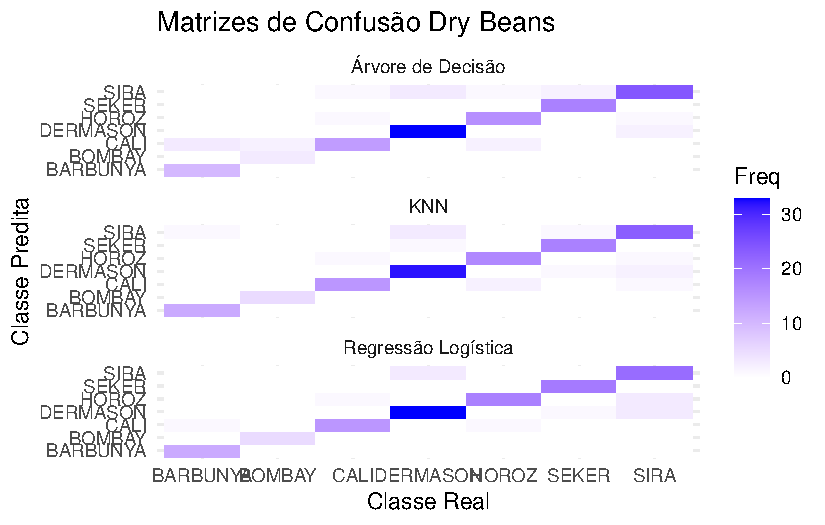
\includegraphics[keepaspectratio]{trabalho_files/figure-pdf/unnamed-chunk-29-1.pdf}}

No Dry Beans, observou-se que a Regressão Logística apresentou o melhor
desempenho em termos de acurácia, seguida pelo KNN e, por último, pela
Árvore de Decisão. Esse resultado pode ser explicado pela natureza dos
atributos do conjunto: as variáveis correspondem a medidas geométricas e
fatores de forma já derivados, muitos deles fortemente correlacionados e
próximos de uma relação linear com as classes. A regressão logística,
por ser um modelo paramétrico, consegue explorar bem essas relações
globais quando há grande quantidade de dados, além de se beneficiar da
padronização aplicada no pré-processamento, o que favorece a
convergência do modelo.

O KNN obteve desempenho intermediário. Isso se deve ao fato de que o
algoritmo depende fortemente da proximidade entre instâncias, e no caso
de variedades de feijão com características muito semelhantes, os
vizinhos podem pertencer a classes diferentes, o que aumenta o número de
erros. Ainda assim, o KNN se mostrou competitivo, principalmente porque
a normalização min--max aplicada no pré-processamento garantiu que todos
os atributos contribuíssem de forma equilibrada no cálculo das
distâncias.

A Árvore de Decisão foi o algoritmo com menor desempenho. O motivo
principal é que esse classificador tende a criar divisões
eixos-paralelas no espaço dos atributos, o que não é suficiente para
capturar fronteiras de decisão mais sutis e contínuas, como as que
distinguem variedades de feijão. Embora valores menores de \emph{cp}
tenham aumentado a complexidade da árvore e melhorado levemente os
resultados, o modelo ainda permaneceu inferior aos demais.

\subsection{Glass Identification
Dataset}\label{glass-identification-dataset-2}

\begin{Shaded}
\begin{Highlighting}[]
\CommentTok{\# {-}{-}{-}{-}{-}{-}{-}{-}{-}{-}{-}{-}{-}{-}{-}{-}{-}{-}{-}{-} Acurácia {-}{-}{-}{-}{-}{-}{-}{-}{-}{-}{-}{-}{-}{-}{-}{-}{-}{-}{-}{-}}
\NormalTok{comparative\_table\_glass }\OtherTok{\textless{}{-}} \FunctionTok{data.frame}\NormalTok{(}
  \AttributeTok{Dataset =} \StringTok{"Glass Identification"}\NormalTok{,}
  \AttributeTok{Classificator =} \FunctionTok{c}\NormalTok{(}\StringTok{"Árvore de Decisão"}\NormalTok{, }\StringTok{"KNN"}\NormalTok{, }\StringTok{"Regressão Logística"}\NormalTok{),}
  \AttributeTok{Accuracy =} \FunctionTok{c}\NormalTok{(acc\_p2\_dt\_glass,acc\_k\_p1\_knn\_glass, acc\_rl\_glass)}
\NormalTok{)}

\NormalTok{comparative\_table\_glass}
\end{Highlighting}
\end{Shaded}

\begin{verbatim}
               Dataset       Classificator  Accuracy
1 Glass Identification   Árvore de Decisão 0.7027027
2 Glass Identification                 KNN 0.7297297
3 Glass Identification Regressão Logística 0.6216216
\end{verbatim}

\begin{Shaded}
\begin{Highlighting}[]
\CommentTok{\# {-}{-}{-}{-}{-}{-}{-}{-}{-}{-}{-}{-}{-}{-}{-}{-}{-}{-}{-}{-} Matriz de Confusão {-}{-}{-}{-}{-}{-}{-}{-}{-}{-}{-}{-}{-}{-}{-}{-}{-}{-}{-}{-}}

\CommentTok{\# Extrair os dados da matriz de confusão e definir modelos}
\NormalTok{cm\_dt\_glass }\OtherTok{\textless{}{-}} \FunctionTok{as.data.frame}\NormalTok{(conf\_p2\_dt\_glass}\SpecialCharTok{$}\NormalTok{table)}
\NormalTok{cm\_dt\_glass}\SpecialCharTok{$}\NormalTok{model }\OtherTok{\textless{}{-}} \StringTok{"Árvore de Decisão"}

\NormalTok{cm\_knn\_glass }\OtherTok{\textless{}{-}} \FunctionTok{as.data.frame}\NormalTok{(conf\_k\_p1\_knn\_glass}\SpecialCharTok{$}\NormalTok{table)}
\NormalTok{cm\_knn\_glass}\SpecialCharTok{$}\NormalTok{model }\OtherTok{\textless{}{-}} \StringTok{"KNN"}

\NormalTok{cm\_rl\_glass }\OtherTok{\textless{}{-}} \FunctionTok{as.data.frame}\NormalTok{(conf\_rl\_glass}\SpecialCharTok{$}\NormalTok{table)}
\NormalTok{cm\_rl\_glass}\SpecialCharTok{$}\NormalTok{model }\OtherTok{\textless{}{-}} \StringTok{"Regressão Logística"}

\CommentTok{\# Combinar as matrizes de confusão}
\NormalTok{cm\_glasss }\OtherTok{\textless{}{-}} \FunctionTok{rbind}\NormalTok{(cm\_dt\_glass, cm\_knn\_glass, cm\_rl\_glass)}

\FunctionTok{ggplot}\NormalTok{(cm\_glasss, }\FunctionTok{aes}\NormalTok{(}\AttributeTok{x =}\NormalTok{ Reference, }\AttributeTok{y =}\NormalTok{ Prediction, }\AttributeTok{fill =}\NormalTok{ Freq)) }\SpecialCharTok{+}
  \FunctionTok{geom\_tile}\NormalTok{() }\SpecialCharTok{+}
  \FunctionTok{facet\_wrap}\NormalTok{(}\SpecialCharTok{\textasciitilde{}}\NormalTok{ model, }\AttributeTok{ncol =} \DecValTok{1}\NormalTok{) }\SpecialCharTok{+} \CommentTok{\# força 1 coluna → todas as matrizes embaixo da outra}
  \FunctionTok{scale\_fill\_gradient}\NormalTok{(}\AttributeTok{low =} \StringTok{"white"}\NormalTok{, }\AttributeTok{high =} \StringTok{"blue"}\NormalTok{) }\SpecialCharTok{+}
  \FunctionTok{theme\_minimal}\NormalTok{() }\SpecialCharTok{+}
  \FunctionTok{labs}\NormalTok{(}
    \AttributeTok{title =}\StringTok{"Matrizes de Confusão Glass Identification"}\NormalTok{,}
    \AttributeTok{x =} \StringTok{"Classe Real"}\NormalTok{,}
    \AttributeTok{y =} \StringTok{"Classe Predita"}
\NormalTok{  )}
\end{Highlighting}
\end{Shaded}

\pandocbounded{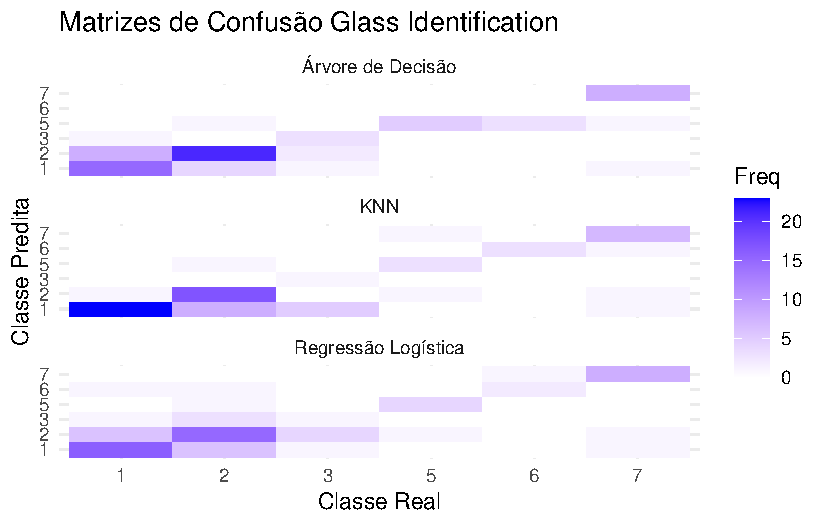
\includegraphics[keepaspectratio]{trabalho_files/figure-pdf/unnamed-chunk-31-1.pdf}}

No Glass, a ordem de desempenho se inverteu parcialmente: o KNN
apresentou a maior acurácia, seguido pela Árvore de Decisão, e por
último a Regressão Logística. Esse comportamento está relacionado às
características da base, que é pequena (214 instâncias), desbalanceada e
com classes muito próximas em termos de composição química.

O KNN apresentou a melhor performance porque o método lida bem com
padrões locais, aproveitando a proximidade entre instâncias semelhantes
mesmo em um espaço não linear. Em bases pequenas como o Glass, a
ausência de suposições paramétricas faz com que o KNN consiga se adaptar
melhor a regiões complexas do espaço de atributos, desde que os dados
estejam normalizados.

A Árvore de Decisão obteve desempenho intermediário, superando a
Regressão Logística. Isso se deve ao fato de que árvores conseguem
capturar interações não lineares entre os atributos químicos, formando
divisões que refletem combinações específicas de valores. Contudo, a
limitação de profundidade e a sensibilidade a ruídos ainda reduzem seu
desempenho em relação ao KNN.

A Regressão Logística, por sua vez, apresentou o pior desempenho no
Glass. A baixa acurácia pode ser atribuída ao tamanho reduzido do
conjunto e à natureza das classes: as fronteiras entre tipos de vidro
dificilmente são lineares, o que limita a capacidade do modelo de
separar adequadamente as categorias. Além disso, o desbalanceamento das
classes aumenta a instabilidade dos coeficientes estimados, mesmo após a
padronização das variáveis.

\subsection{Comparação Geral e
Implicações}\label{comparauxe7uxe3o-geral-e-implicauxe7uxf5es}

Os resultados mostram que não existe um único algoritmo superior em
todos os contextos; o desempenho depende das características do conjunto
de dados. Em bases grandes, com atributos derivados e relações mais
próximas da linearidade, como no Dry Beans, a Regressão Logística se
mostrou a mais eficaz. Já em bases pequenas e com fronteiras de decisão
complexas, como no Glass, métodos não paramétricos (KNN e Árvore)
superaram a RL.

Além disso, o estudo evidencia a importância do pré-processamento: a
normalização (re-escala para KNN e padronização para RL) foi essencial
para que os algoritmos funcionassem adequadamente, e a redução de
dimensionalidade no Dry Beans contribuiu para reduzir redundâncias,
melhorando o desempenho dos modelos.

Esses achados estão em consonância com a teoria de aprendizado de
máquina: modelos paramétricos tendem a ser favorecidos em conjuntos
grandes e bem estruturados, enquanto modelos baseados em vizinhança ou
árvores se beneficiam quando o espaço de decisão é mais irregular ou
quando há poucos dados disponíveis.




\end{document}
